\chapter{Landslide}
\label{chap:landslide}

\inspirationalquote{Somewhere is the promise of an uncharted trail, with 700 branching limbs and 700 ways to fail.}
{ThouShaltNot, Cardinal Directions}

Landslide is a model checker implemented as a plug-in module for x86 full-system simulators.
The program to be tested runs in a simulated environment,
and Landslide uses its access to the simulator's internal state to inspect and manipulate the memory and thread scheduling of the program as it executes.
As of this thesis's writing, Landslide supports the use of two possible simulators:

\begin{itemize}
	\item {\bf Simics} \cite{simics}, a proprietary simulator licensed commercially by Wind River, used at CMU in 15-410 to run Pebbles thread libraries and kernels, and
	\item {\bf Bochs} \cite{bochs}, an open-source (LGPL) simulator used at the University of Chicago, Berkeley, Stanford, and other schools to run Pintos kernels.
\end{itemize}

% TODO: add some backup linkeroos
The Bochs port of Landslide is likewise open-source
\revisionminor{under the \landslidelicense license}
and available at \url{https://github.com/bblum/landslide}.
% TODO: refresh
The HEAD commit at the time of writing is 8127151.
The Simics port uses Simics's proprietary API and is hence unlicensed and available upon request for educational use only.
Development on the Simics port is largely frozen,
as the Bochs port implements all the same features and more,
and is also roughly 3x faster.

This chapter will discuss Landslide's outer and inner workings in all their gory detail.
It is intended for the aspiring developer or the ambitious user
and hence unlike other chapters is written in the style of documentation rather than as a report of research results.
The reader interested only in a theoretical introduction to model checking's foundational algorithms,
with detailed and friendly examples to help establish intuitions the later chapters may require,
may skip to \cref{sec:landslide-algs}.

%%%%%%%%%%%%%%%%%%%%%%%%%%%%%%%%%%%%%%%%%%%%%%%%%%%%%%%%%%%%%%%%%%%%%%%%%%%%%%%%
%%%%%%%%%%%%%%%%%%%%%%%%%%%%%%%%%%%%%%%%%%%%%%%%%%%%%%%%%%%%%%%%%%%%%%%%%%%%%%%%
%%%%%%%%%%%%%%%%%%%%%%%%%%%%%%%%%%%%%%%%%%%%%%%%%%%%%%%%%%%%%%%%%%%%%%%%%%%%%%%%

\section{User interface}

This section describes the features of Landslide the average student user should expect to interact with.
% TODO: make more specific section reference
Separate user guides also exist, described in \Cref{chap:education}.

%%%%%%%%%%%%%%%%%%%%%%%%%%%%%%%%%%%%%%%%%%%%%%%%%%%%%%%%%%%%%%%%%%%%%%%%%%%%%%%%

\subsection{Setup}
\label{sec:landslide-setup}

Three setup scripts are provided, one for each supported kernel architecture: {\tt p2-setup.sh}, {\tt psu-setup.sh}, and {\tt pintos-setup.sh}.
The user should supply the directory containing her project implementation.
The second of the three is largely the same as the first, with CMU-specific project details replaced by PSU-specific ones.
The latter of the three also supports arguments specifying which of the Pintos projects to target.
For example:
\begin{itemize}
	\item {\tt ./p2-setup.sh /path/to/my/p2}
	\item {\tt ./psu-setup.sh /path/to/my/thrlib}
	\item {\tt ./pintos-setup.sh /path/to/my/threads} (2nd argument defaults to ``{\tt threads}'')
	\item {\tt ./pintos-setup.sh /path/to/my/userprog userprog}
\end{itemize}

These scripts accomplish the following setup tasks (among other trivialities):
\begin{itemize}
	\item Copy the user's code into {\tt pebsim/p2-basecode/} or {\tt pebsim/pintos/},
		which contain a pre-annotated Pebbles reference kernel binary or pre-annotated Pintos basecode, respectively.
	\item Build the code in its new location.
	\item Run the instrumentation script on the resulting binary to let Landslide know where all the important functions are
		(see \cref{sec:landslide-glue}).
\end{itemize}

%%%%%%%%%%%%%%%%%%%%%%%%%%%%%%%%%%%%%%%%%%%%%%%%%%%%%%%%%%%%%%%%%%%%%%%%%%%%%%%%

\subsection{Running Landslide through Quicksand}
\label{sec:landslide-quicksand-options}

The preferred method of invoking Landslide is through Quicksand, the Iterative Deepening wrapper program which has all of \Cref{chap:quicksand} to itself.
% TODO: add quicksand symlink
This is done via the {\tt ./landslide} script in the top-level directory, which:
\begin{itemize}
	\item Checks if the user needs to run {\tt *-setup.sh} again, in case her source code was more recently updated than the existing annotated build (a common mistake),
	\item Passes its arguments through to {\tt id/landslide-id}, the Quicksand binary,
		and
	\item (If during the student user study,) compresses the resulting log files,
		creates a snapshot tarball of them and the current version of the user's code,
		and sends it to me for nefarious research purposes
		\revisionminor{(see \cref{sec:education-pebbles-instrumentation})}.
\end{itemize}

%%%%%%%%%%%%%%%%%%%%%%%%%%%%%%%%%%%%%%%%%%%%%%%%%%%%%%%%%%%%%%%%%%%%%%%%%%%%%%%%

\subsubsection{Command-line argments}

The following command line arguments are recommended for the common user.

\begin{itemize}
	\item {\tt -p PROGRAM}: the name of the test case to invoke
	\item {\tt -t TIME}: wall-clock time limit, in seconds; or suffixed with one of {\tt ydhms} for years, days, hours, minutes, or seconds respectively (default 1h)
	\item {\tt -c CPUS}: maximum number of Landslide instances to run in parallel (defaults to half the number of system CPUs)
	\item {\tt -i INTERVAL}: interval of time between printing progress reports (default 10s)
	\item {\tt -d TRACEDIR}: directory for resulting bug traces (default current directory)
	\item {\tt -v}: verbose mode (issues output for each executed interleaving by each instance of landslide, makes progress reports more detailed, etc)
	\item {\tt -l}: leave Landslide log files from completed state spaces even when no bug was found (deleted automatically by default)
	\item {\tt -h}: print help text and exit immediately
	\item \revision{{\tt -s}: include ``secret'' options when printing help text}
\end{itemize}

The following ``secret'' arguments also exist, primarily for my own use in running experiments or debugging.

\begin{itemize}
	\item {\tt -C}: enable ``control experiment'' mode, i.e., run only 1 instance of Landslide, with all (non-data-race) preemption points enabled in advance
		% TODO: put a section reference here
	\item {\tt -I}: enable Iterative Context Bounding (requires {\tt -C}, although future work may relax this restriction);
		this generally causes bugs to be found faster should they exist, but degrades completion time
		(\cref{sec:landslide-icb})
	\item {\tt -0}: enable Preempt-Everywhere mode (\cref{sec:quicksand-eval}, requires {\tt -C})
	\item {\tt -M}: enable Maximal State Space mode,
		which prioritizes the maximal state space to optimize for fast verification,
		abandoning all subset jobs even if they might find bugs faster
		(\cref{sec:tm-eval}, incompatible with {\tt -C}).
		According to \cref{sec:quicksand-soundness}'s soundness proofs,
		this is equivalent to {\tt -0}
		(and according to my experience, \revisionminor{much} faster as well).
	\item {\tt -H}: use Limited Happens-Before for data-race analysis (\cref{sec:background-hb})
		(default for Pebbles kernelspace mode)
	\item {\tt -V}: use vector-clock-based Pure Happens-Before for data-race analysis (\cref{sec:background-hb})
		(default for P2/PSU userspace and Pintos modes)
	\item {\tt -X}: support transactional memory (\Cref{chap:tm})
	\item {\tt -A}: support multiple abort codes during transaction failure (\cref{sec:tm-implementation});
		required for testing programs which behave differently under different abort circumstances,
		but impacts the state space size
	\item {\tt -S}: suppress retry aborts during transaction failure (\cref{sec:tm-implementation})
	\item {\tt -R}: enable retry-set state space reduction for transactional tests (\cref{sec:tm-implementation})
	\item {\tt -P}: support Pintos architecture (enabled automatically when {\tt pintos-setup.sh} is run)
	\item {\tt -4}: support Pebbles architecture (enabled automatically when either {\tt p2-setup.sh} or {\tt psu-setup.sh} is run)
		% TODO: put a section reference
	\item {\tt -e ETAFACTOR}: configure heuristic state space ETA deferring factor (described in detail in {\tt id/option.c})
	\item {\tt -E ETATHRESH}: configure heuristic threshold of state space progress for judging ETA stability (described in detail in {\tt id/option.c})
\end{itemize}

Quicksand will automatically generate configuration files and invoke Landslide according to the process described in the next section.

%%%%%%%%%%%%%%%%%%%%%%%%%%%%%%%%%%%%%%%%%%%%%%%%%%%%%%%%%%%%%%%%%%%%%%%%%%%%%%%%

\subsection{Running Landslide directly}
\label{sec:landslide-directly}

Rather than letting Quicksand juggle multiple instances of Landslide,
the user may run a single instance directly, optionally configuring the preemption points by hand.
This is recommended only for the enthusiastic user annotating her own kernel.

The script {\tt pebsim/landslide} invokes Landslide thus.
It should be run from within the {\tt pebsim/} directory.
When supplied no arguments, it reads configuration options from {\tt pebsim/config.landslide}
(a bash script expected to define certain variables as described in \cref{sec:landslide-glue}).
The user may optionally specify a file containing additional config directives
% , such as custom preemption points,
as an argument.\footnote{
Quicksand actually supplies two such files as arguments: one ``static'' config file and one ''dynamic'' config file.
The former contains options which require recompiling Landslide (e.g., whether or not to use ICB is controlled by an {\tt \#ifdef} in Landslide's code),
while the latter contains options which Landslide interprets at runtime (e.g., which preemption points to use).
The static options do not change between Landslide instances in a single Quicksand run,
avoiding long Landslide start-up times.
}
Such supported options are as follows.

\subsubsection{Dynamic configuration options}
\label{sec:landslide-dynamicconfig}

First, the following options may be changed without triggering a recompile of Landslide.
They are implemented as bash functions defined in {\tt pebsim/build.sh}.

\begin{itemize}
	\item {\tt within\_function FUNC} - adds {\tt FUNC} to an allowlist of functions required to appear in the current stack trace before identifying a preemption point (see \cref{sec:landslide-pps})
	\item {\tt without\_function FUNC} - as above, but a denylist instead of an allowlist
	\item {\tt within\_user\_function FUNC} - as two above but finds the function in the userspace test program rather than the kernel code.
	\item {\tt without\_user\_function FUNC} - difference to two above same as stated one above.
	\item {\tt data\_race ADDR TID LAST\_CALL CURRENT\_SYSCALL} - specifies a data-race preemption point.
		\begin{itemize}
			\item {\tt ADDR} shall be the code address (in hex) of the racing address,
			{\em before} the execution of which a preemption will be issued.
			\item {\tt TID} indicates a thread ID required to be running for this data race.
				To specify data race PPs across all threads at once, set {\tt FILTER\_DRS\_BY\_TID=0} (see next section).
			\item {\tt LAST\_CALL} indicates a code address required to be the site of the last {\tt call} instruction executed
				(similar to specifying a stack trace, but using a full stack trace here degrades performance too much),
				or 0 to not use this feature.
				From personal experience I found this option rather useless and recommend always supplying 0.
				% TODO: fix this section ref
				For further discussion see \cref{sec:quicksand-pps}.
			\item {\tt CURRENT\_SYSCALL} indicates the system call number if a user-space data race comes from within a kernel system call which accesses user memory (Pebbles only).
				Usually 0 (i.e., not in kernel code) but {\tt deschedule}'s system call number is common as well.
		\end{itemize}
	\item {\tt input\_pipe FILENAME} - FIFO file used for receiving messages from Quicksand (e.g. to suspend or resume execution).
		Requires {\tt id\_magic} option to be set (next section below).
		The odds that a human user will find spiritual enlightenment through using this option by hand are infinitesimal.
	\item {\tt output\_pipe FILENAME} - as above but for sending messages.
\end{itemize}

\subsubsection{Static configuration options}
\label{sec:landslide-staticconfig}

Next, configuration options which affect an {\tt \#ifdef} in Landslide and will trigger a recompile upon changing.
%These span a wide variety of features, sorted below in subsections by roughly how interesting I think they are.
Unless otherwise specified these are boolean flags (1 or 0) and the example value shown indicates the default used if unspecified.

\begin{itemize}
\item {\bf Search algorithm options}
\begin{itemize}
	\item {\tt ICB=0} - enable Iterative Context Bounding (\cref{sec:landslide-icb});
		corresponds to {\tt -I} in \cref{sec:landslide-quicksand-options}.
	\item {\tt PREEMPT\_EVERYWHERE=0} - enable Preempt-Everywhere mode (\cref{sec:quicksand-eval});
		corresponds to {\tt -0} in \cref{sec:landslide-quicksand-options}.
	\item {\tt EXPLORE\_BACKWARDS=0} - configure whether, at each newly encountered preemption point,
		to allow the current thread to run first then later upon backtracking to preempt (0),
		or to issue preemptions first and then try continuing the current thread later (1).
		0 tends to produce shorter preemption traces while 1 tends to find bugs faster (\cite[\S{}8.7.1]{landslide}).
		Not compatible with ICB.
\end{itemize}

\item {\bf Memory analysis options}
\begin{itemize}
	\item {\tt PURE\_HAPPENS\_BEFORE=1} - select Pure Happens-Before (1) or Limited Happens-Before (2) (\cref{sec:background-hb});
		corresponds to {\tt -V}/{\tt -H} in \cref{sec:landslide-quicksand-options}.
	\item {\tt FILTER\_DRS\_BY\_TID=1} - configures whether to use the {\tt TID} parameter of {\tt data\_\allowbreak{}race} described above.
	\item {\tt FILTER\_DRS\_BY\_LAST\_CALL=0} - configures whether to use the {\tt LAST\_CALL} parameter of {\tt data\_race} described above.
	\item {\tt ALLOW\_LOCK\_HANDOFF=0} - configures lockset tracking to permit or disallow a lock taken by one thread to be released by another thread.%
		\footnote{If enabled, accesses performed by the second thread before unlocking will not be considered protected by that lock,
			as Landslide cannot infer what prior event abstractly represented the lock's ownership changing,
			leading to spurious data race reports.
			This could be solved in future work with a new annotation.}
	\item {\tt ALLOW\_REENTRANT\_MALLOC\_FREE=0} - allow two threads to be in {\tt malloc}, {\tt free}, or so on simultaneously without declaring it a bug.%
		\footnote{Used in Pintos, where those functions lock/unlock the heap mutex themselves rather than relying on a wrapper function to do so before invoking them.}
	\item {\tt TESTING\_MUTEXES=0} - configure ``mutex testing'' mode (1),
		in which the data race analysis will not consider a mutex's implementation to be protected by the mutex itself.
		In other words, the mutex's internal memory accesses will be flagged as data races,
		thereby enabling Landslide to verify the mutual exclusion property.
		Normally (0), Landslide assumes mutual exclusion is provided in order to efficiently find data races in the rest of the code.
		Quicksand will automatically set this option for P2s when {\tt -t mutex\_test} is specified.
\end{itemize}

\item {\bf Interface options}
\begin{itemize}
	\item {\tt TEST\_CASE=NAME} - configure the name of the test program to run (mandatory; no default)
	\item {\tt VERBOSE=0} - enable more verbose output
	\item {\tt BREAK\_ON\_BUG=0} - configure whether to exit the simulator or drop into a debug prompt when a bug is found. Simics only and not compatible with Quicksand.
	\item {\tt DONT\_EXPLORE=0} - if enabled, Landslide will not perform stateless model checking but rather will execute the default thread interleaving then exit (useful for manual inspection of preemption points).
	\item {\tt PRINT\_DATA\_RACES=0} - as it says on the tin (for stand-alone use; will message them to Quicksand regardless).
	\item {\tt TABULAR\_TRACE=1} - configure whether to emit bug reports to the console (0) or to an HTML trace file (1)
\end{itemize}
\end{itemize}

%%%%%%%%%%%%%%%%%%%%%%%%%%%%%%%%%%%%%%%%%%%%%%%%%%%%%%%%%%%%%%%%%%%%%%%%%%%%%%%%

\subsection{Test cases}
\label{sec:landslide-testcases}

Landslide depends on human intuition to construct a test case
that will produce both meaningful in quality and manageable in quantity thread interleavings.

The user may supply custom test cases
for Pebbles (under {\tt pebsim/p2-basecode})
by creating a file in {\tt 410user/progs} and adding it to config.mk as usual,
or for Pintos (under {\tt pebsim/pintos/src/tests/threads})
by creating a file and adding it to both {\tt tests.c} and {\tt Make.tests}.
Tests for the most common interactions during the P2 and Pintos projects are of course already supplied,
as described in \cref{sec:education-pebbles-tests} and \cref{sec:education-pintos-tests}.

Use of {\tt tell\_landslide()} annotations
\revisionminor{(\cref{sec:tell-landslide})}
is not necessary,
although {\tt tell\_landslide\_\allowbreak{}preempt()} and {\tt tell\_landslide\_dump\_stack()}
may optionally be used at the user's convenience.
Additionally, the following ``secret'' annotations
are occasionally used in the pre-supplied test cases
to accomplish several mysterious goals described hereupon.

\subsubsection{Magic post-test assertions}

Test cases may define global variables of the following names
to instruct Landslide to assert the following corresponding predicates at the end of each test execution,
after all threads exit.
Each predicate will be checked iff its first listed variable name is defined;
if that variable is defined, all others associated must also be;
any combination of the three first-listed variables may be specified at the user's option.
\begin{itemize}
	\item {\tt magic\_global\_expected\_result == magic\_global\_value}
	\item {\tt magic\_expected\_sum == magic\_thread\_local\_value\_parent +} \\ {\tt magic\_thread\_local\_value\_child}
	\item {\tt magic\_expected\_sum\_minus\_result == magic\_thread\_local\_value\_parent +} \\ {\tt magic\_thread\_local\_value\_child - magic\_global\_value}
\end{itemize}
\revision{Because Landslide tests the ultimate value of these variables after all threads have completed execution,}
these could not be implemented as asserts in the test code itself
without requiring the student to implement {\tt thr\_join()} and {\tt thr\_exit()},
avoiding which is important for tests to be student-accessible earlier in the project implementation timeline.

\subsubsection{Misbehave}
\label{sec:landslide-friendly-misbehave}

Many of the supplied P2 test cases invoke the {\tt misbehave} system call
with a mysterious argument (usually {\tt BGND\_BRWN >> FGND\_CYAN})
before the creation of any child threads.
The use of terminal color code constants is of course a red herring of obfuscation,
as the true nature of the Pathos reference kernel's {\tt misbehave} modes
is a closely-guarded secret among 15-410 course staff (\cref{sec:410-secrecy}).
The mode in question causes the reference kernel to prioritize scheduling the child thread over the parent
whenever {\tt thread\_fork} is called,
and the target thread over the invoking thread
whenever {\tt make\_runnable} is called,
which are necessary to allow Landslide to recognize a {\tt yield()} preemption point
and be able to run the newly-runnable thread as soon as possible.

To illustrate, consider the following program in \Cref{fig:misbehave-example},
and suppose Landslide is configured to preempt only on mutex API calls
(such as in the first step of Iterative Deepening (\cref{sec:quicksand-id})).
Because Landslide ignores all kernel-level synchronization short of context switches when testing user-level code,
if the kernel created the child thread and returned from {\tt thread\_fork}
(the system call underlying {\tt thr\_create()})
without yielding first,
the next preemption point will not occur until {\tt thr\_join()} waits for the child to exit.
Hence, DPOR will erroneously think everything before that {\tt thr\_join()}
happens-before (\cref{sec:landslide-dpor-hb}) anything the child does,
and will fail to identify the racing accesses on {\tt x}.

\begin{figure}[h]
	\begin{center}
	\begin{tabular}{l}
		\texttt{\ctype{void} \call{child}(\ctype{int} *xp) \{} \\
		\texttt{~~~~*xp++;} \\
		\texttt{\}} \\
		\\
		\texttt{\ctype{void} \call{parent}() \{} \\
		\texttt{~~~~\ctype{int} x = \const{0};} \\
		\texttt{~~~~\ctype{int} tid = \call{thr\_create}(child, \&x);} \\
		\texttt{~~~~x++;} \\
		\texttt{~~~~\call{thr\_join}(tid, \const{NULL});} \\
		\texttt{~~~~\flow{assert}{}(x == \const{2});} \\
		\texttt{\}} \\
	\end{tabular}
	\end{center}
	\caption[Example demonstrating the need for {\tt misbehave}.]
		{Example demonstrating the need for {\tt misbehave} to force the kernel
	to yield during {\tt thread\_fork}.}
	\label{fig:misbehave-example}
\end{figure}

Though Iterative Deepening's soundness (\cref{sec:quicksand-soundness})
guarantees all data races will eventually be detected starting from just synchronization preemption points,
it assumes threads becoming runnable counts among those.
In that sense, {\tt misbehave} serves to restore the last synchronization preemptions where they belong.
If at this point the reader wonders why Landslide doesn't just identify
the {\tt thread\_create} and {\tt make\_runnable} system calls in the arbiter itself (\cref{sec:landslide-arbiter})
and skip this mysterious user-visible complexity,
they would be right to ask:
I have left it this way for no better reason than to maintain consistency
with the upcoming chapters' experimental environments,
and intend on fixing it in a future update.

Other {\tt misbehave} modes may be used, but are likely to have no effect,
since Landslide's thread-scheduling algorithm will override
any Pathos-internal scheduling priorities that may arise therefrom.
Hypothetically speaking, a reader with access to the top-secret Pathos source code
could find further {\tt misbehave} documentation in its {\tt inc/misbehavior.h}.

%%%%%%%%%%%%%%%%%%%%%%%%%%%%%%%%%%%%%%%%%%%%%%%%%%%%%%%%%%%%%%%%%%%%%%%%%%%%%%%%

\subsection{Bug reports}
\label{sec:landslide-bugreport}

When Landslide finds a bug, it produces an execution trace of the particular interleaving of threads that led to the bug.
This takes the form of a two-dimensional table,
with a column for each thread,
and each row representing the continuous execution of one thread between two (not necessarily consecutive) preemption points.
In each row, the cell in the column corresponding to the executed thread will contain a stack trace,
indicating the code location of the preemption point {\em at the end} of that thread transition
(i.e., each stack trace indicates ``this thread ran until it reached the indicated line of code'').
The bug reports are formatted in \revisionminor{HTML}, recommended to be viewed in a web browser.
An example is shown in \Cref{fig:bugreport}.

In addition to the preemption trace, the bug report provides some additional helpful information:
a stack trace of the current thread at the ultimate point when the bug was executed
\revision{(the same as the stack trace in the cell corresponding to that thread in the bottom row of the table)},
a message indicating the nature of the bug encountered,
statistics about the size of the state space,
and optionally additional information about the bug.%
\footnote{For certain types of bugs, not pictured here;
for example, use-after-frees will report separate stack traces
indicating when the corresponding heap block was last allocated and freed.
The intrepid source-diver may find all such cases of extra bug details
by searching for the macro {\tt FOUND\_A\_BUG\_HTML\_INFO} in Landslide's code.}
\revision{\cref{sec:future-friendly} discusses how these bug reports might be further improved
by adding more information still,
such as identifying data-race preemption points or listing memory conflicts that occurred during each transition.}

% TODO: check figure placement
\begin{figure}[h!]
	\begin{center}
		% XXX: at 0.986\textwidth or bigger, latex puts this infinity pages into the future
		% at 0.985 or lower, it goes on the right page
		% wtffff latex.
		% nb. generated from landslide-trace-1506524837.14.html
		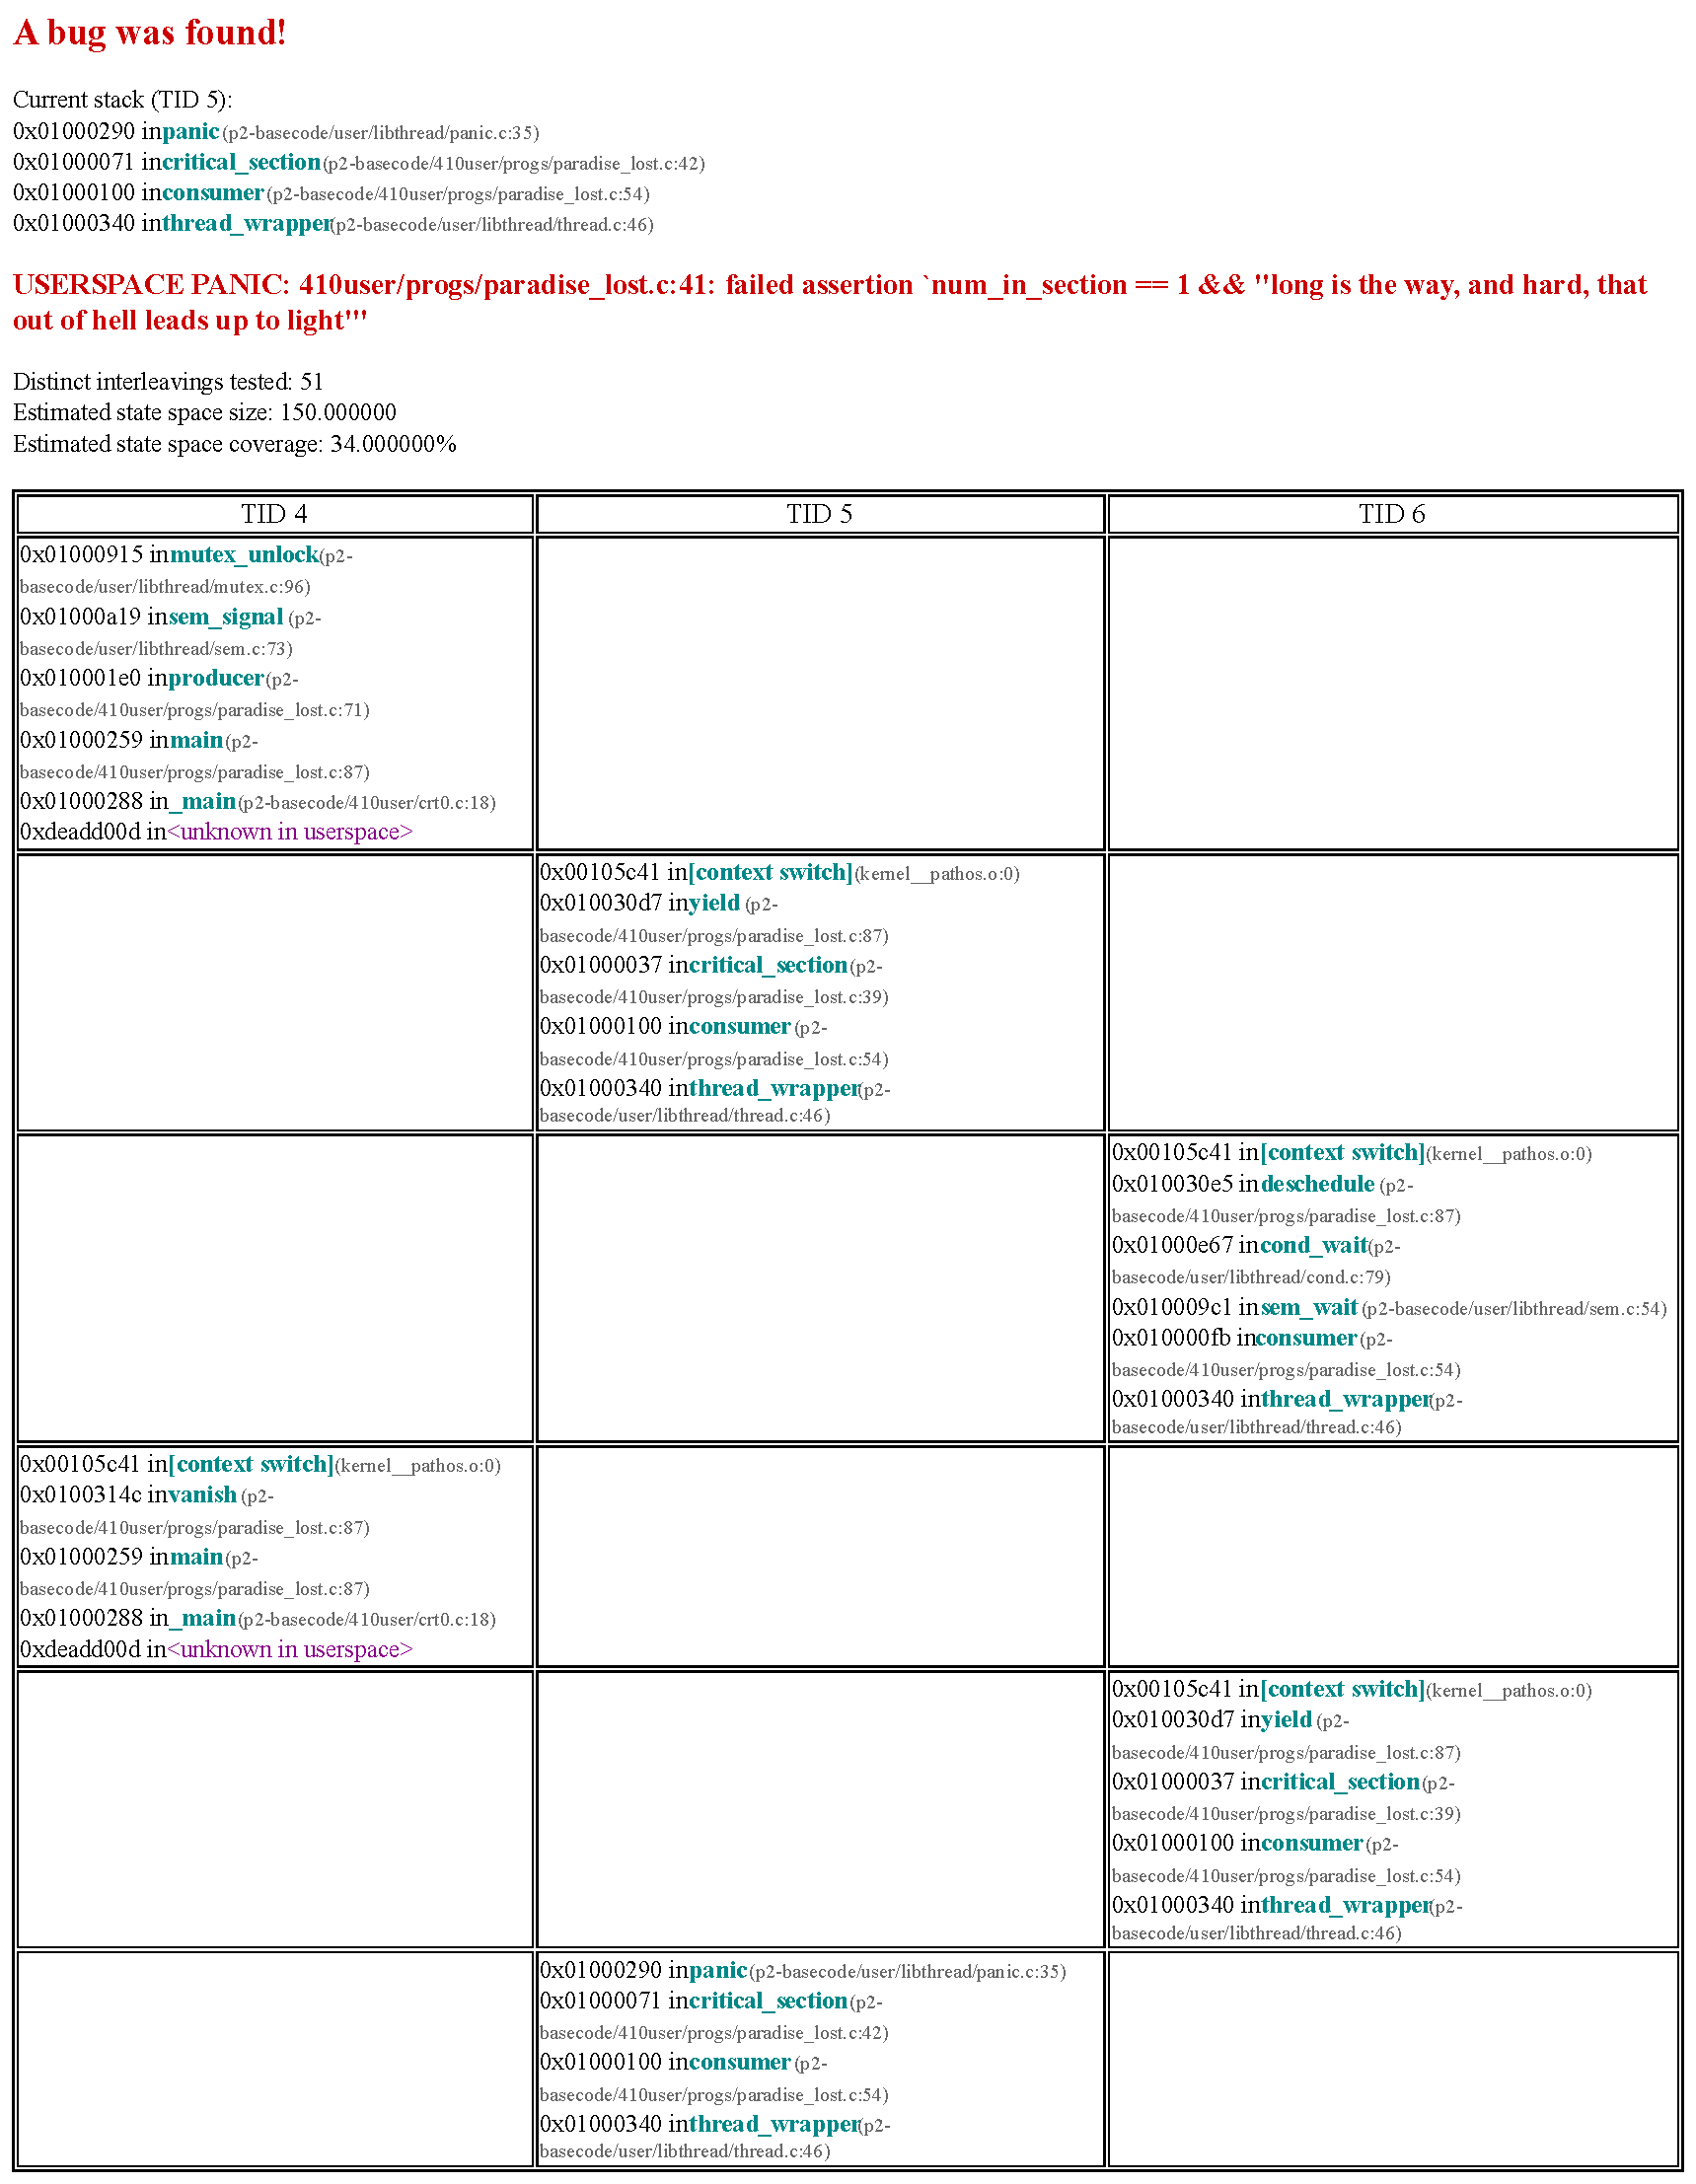
\includegraphics[width=0.985\textwidth]{bugreport.pdf}
	\end{center}
	\caption{Example preemption trace bug report.}
	\label{fig:bugreport}
\end{figure}

%%%%%%%%%%%%%%%%%%%%%%%%%%%%%%%%%%%%%%%%%%%%%%%%%%%%%%%%%%%%%%%%%%%%%%%%%%%%%%%%
%%%%%%%%%%%%%%%%%%%%%%%%%%%%%%%%%%%%%%%%%%%%%%%%%%%%%%%%%%%%%%%%%%%%%%%%%%%%%%%%
%%%%%%%%%%%%%%%%%%%%%%%%%%%%%%%%%%%%%%%%%%%%%%%%%%%%%%%%%%%%%%%%%%%%%%%%%%%%%%%%

\section{Kernel annotations}

\revision{My M.S. thesis \cite{landslide}
investigated the annotation overhead required for a user to instrument a Pebbles kernel for use with Landslide.
On average, students who volunteered for the study (conducted during P3) required 2 hours for this process.
While many of these students then went on to find and diagnose bugs,
this was deemed an unacceptable burden for an educational tool to impose on struggling students.
%(as opposed to those who had enough free time and ambition to volunteer for a study
%that was advertised in advance as requiring manual annotations)

Hence,}
the educational experiments in this thesis focus on projects which students implement
on top of provided kernel basecode which Landslide already ``understands''.
Such understanding is conferred via the annotations described in this section.
For P2 and Pintos students I supply these annotations behind the scenes,
but a CMU 15-410 student who wishes to use Landslide on her kernel project shall need to brave forth hereupon.

%%%%%%%%%%%%%%%%%%%%%%%%%%%%%%%%%%%%%%%%%%%%%%%%%%%%%%%%%%%%%%%%%%%%%%%%%%%%%%%%

\subsection{config.landslide annotations}
\label{sec:landslide-config-landslide}

The following annotations are specified in {\tt pebsim/config.landslide} akin to the static configuration options
described in \cref{sec:landslide-directly}.
These specify the names of kernel functions, global variables, default values, and so on
which are required to accurately track the kernel's scheduler state:
{\tt CONTEXT\_SWITCH},
{\tt EXEC},
{\tt FIRST\_TID},
{\tt IDLE\_TID},
{\tt INIT\_TID},
{\tt MEMSET},
{\tt PAGE\_FAULT\_WRAPPER},
{\tt READLINE},
{\tt SFREE},
{\tt SHELL\_TID},
{\tt SPURIOUS\_INTERRUPT\_WRAPPER},
\\
{\tt THREAD\_KILLED\_ARG\_VAL},
{\tt THREAD\_KILLED\_FUNC},
{\tt TIMER\_WRAPPER},
{\tt VM\_USER\_COPY},
\\
{\tt VM\_USER\_COPY\_TAIL},
{\tt YIELD}.

Following are the less self-explanatory options.
\revision{Those defined with an equals sign between name and value
are implemented as bash variables,
which the annotation scripts check after processing the configuration to emit a corresponding {\tt \#define}
within Landslide itself;
those defined with no equals sign
are implemented as bash functions,
which the annotation scripts define in advance of processing the configuration to do something more complicated.}
\begin{itemize}
	\item {\tt PINTOS\_KERNEL=0} - configure Landslide for Pebbles (0) or Pintos (1) kernel architecture. Normally set automatically by the setup scripts.
	\item {\tt TESTING\_USERSPACE=1} - configure Landslide whether to test (i.e., focus preemption points, memory analysis, etc. on) the userspace or kernelspace code.
	\item {\tt CURRENT\_THREAD\_LIVES\_ON\_RQ=0} - Landslide infers the list of runnable threads from the {\tt tell\_landslide\_on\_rq()} and {\tt off\_rq()} annotations (described below).
		Some kernels\footnote{Most, actually.} remove the current thread from their runqueue,
		such that the abstract set of all runnable threads is actually the runqueue plus the current thread rather than just the runqueue.
		Other kernels\footnote{The author's own student kernel from long ago.}
		leave the current thread on the runqueue,
		removing it only when it's descheduling and should actually be considered blocked.
		Set this option to 0 to support the former kernel type or 1 to support the latter.%
		\footnote{This option replaces the deprecated {\tt kern\_current\_extra\_runnable()} annotation from {\tt student.c} described in \cite[\S{}6.2.3]{landslide}.}
		\revision{Whether or not a kernel requires this annotation could be auto-detected in future work.}
	\item {\tt PREEMPT\_ENABLE\_FLAG=NAME} - name of a global variable which the kernel uses to toggle scheduler preemptability, for kernels which may disable preemption without disabling interrupts.
		For kernels wherein preemptability is corresponds directly by interrupts, leave this option unspecified.
	\item {\tt PREEMPT\_ENABLE\_VALUE=VAL} - value of the above variable when preemption is enabled
		(usually 0; note that many kernels use a nesting depth counter where any positive value corresponds to disabled).%
		\footnote{These two options replace the deprecated {\tt kern\_ready\_for\_timer\_interrupt()} annotation from {\tt student.c} described in \cite{landslide} \sect{6.2.3}.}
	\item {\tt PATHOS\_SYSCALL\_IRET\_DISTANCE=VALUE} - indicate how much stack space is used by the reference kernel's system call wrappers.
		Used for cross-kernel-to-userspace stack traces;
		if unset, stack traces from kernel space will end at the system call boundary.
	\item {\tt PDE\_PTE\_POISON=VALUE} - indicate a poison value used in the page tables to indicate absent VM mappings to check for as well as checking the present bit (if unspecified, will check present bit only)
	\item {\tt BUG\_ON\_THREADS\_WEDGED=1} - set to 0 to disable deadlock detection but instead let the kernel keep receiving system interrupts when all threads appear blocked.%
		\footnote{Once used in the bad old days; now recommended for debugging use only.}
	\item {\tt TIMER\_WRAPPER\_DISPATCH=NAME} - used to manually indicate a label before the end of the timer interrupt assembly wrapper, in case the {\tt iret} instruction couldn't be found automatically (see {\tt pebsim/definegen.sh}).
	\item {\tt starting\_threads TID STARTS\_ON\_RQ} - specifies a system thread which already exists at the time {\tt tell\_landslide\_sched\_init\_done()} (see below) is called; {\tt TID} is the thread's ID and {\tt STARTS\_ON\_RQ} is 0 or 1 to indicate whether or not it starts on the system runqueue.
		Typical threads to use this for are init and idle.
	\item {\tt ignore\_sym NAME SIZE} - specifies a global variable {\tt NAME} of a given {\tt SIZE} in bytes whose memory accesses should be ignored for the purposes of DPOR and data race analysis.
		Typical symbols to use this for are the console or heap mutex.
	\item {\tt sched\_func NAME} - specifies a function whose memory accesses should all be ignored for the purposes of DPOR and data race analysis.
		Typical functions to use this for are the timer handler and context switcher.
	\item {\tt disk\_io\_func NAME} - specifies a function which may block a thread waiting for disk I/O (or other external interrupt) rather than blocking on another thread.
		If any threads are blocked in a disk I/O function during an apparent deadlock,
		Landslide will allow the kernel to idle until the simulator delivers the appropriate interrupt,
		rather than declaring a bug.
	\item {\tt ignore\_dr\_function NAME USERSPACE} - specifies a function whose memory access should not be counted as data races (but still be considered memory conflicts for DPOR).
		{\tt USERSPACE} should be 0 or 1 to denote a kernel-space or user-space function respectively.
	\item {\tt thrlib\_function NAME} - specifies a function whose memory accesses should be ignored both by the data race analysis and by DPOR.
		This is recommended for marking trusted-correct thread library code when testing multithreaded client code thereof,
		in order to avoid unnecessarily checking, for example,
		all the different ways {\tt thr\_exit()} and {\tt thr\_join()} could interleave.
		The user should be careful with this option to also enable the proper {\tt thr\_create()} misbehave mode
		in her test case (\cref{sec:landslide-friendly-misbehave}).
	\item {\tt TRUSTED\_THR\_JOIN=0} - if set to 1, forces Landslide to add a happens-before edge (\cref{sec:landslide-dpor-hb}) between the exiting of some thread $N$ and the end of any subsequent {\tt thr\_join}$(N)$ call,
		even if that {\tt join} would not ordinarily block.
		This is useful for state space reduction when testing threaded client code;
		for example,
		in the interleaving
		TID1: {\tt x++; thr\_exit();},
		TID2: {\tt thr\_join(1); print(x);},
		%this {\tt join} will wait on no condition variables, just take a few uncontended mutexes, reap the thread,
		%and go along on its way, so
		DPOR, not automatically trusting {\tt join}'s behaviour,
		will attempt to test the TID2, TID1 interleaving to reorder the accesses on {\tt x},
		whereupon {\tt join} will block, forcing these interleavings to be equivalent.
		% if you had tested them in the other order to begin with, dpor would detect this dependency,
		% and would skip the other equivalent interleaving
		This option allows DPOR to skip checking that {\tt join} behaves properly
		and to prune the second interleaving
		by teaching it the expected blocking semantics. %to begin with.
		Obviously, not for use when actually testing {\tt thr\_join} itself!
\end{itemize}

%%%%%%%%%%%%%%%%%%%%%%%%%%%%%%%%%%%%%%%%%%%%%%%%%%%%%%%%%%%%%%%%%%%%%%%%%%%%%%%%

\subsection{In-kernel code annotations}
\label{sec:tell-landslide}

The following annotations are provided as C functions
which a kernel author shall include in her source code and call at appropriate times.
The functions' actual implementations are empty;
rather they serve as labels whose positions the annotation scripts extract
along with the other various annotations from the previous section.
Some of these are mandatory for Landslide to function properly,
while others serve to improve or otherwise manipulate the state space.

\subsubsection{Mandatory annotations}

\begin{itemize}
	\item {\tt tell\_landslide\_thread\_switch(int new\_tid)} - to be called during context switch, indicating the newly-running thread
		(must be called with interrupts and/or scheduler preemption disabled)
	\item {\tt tell\_landslide\_sched\_init\_done()} - to be called after scheduler initialization,
		indicating the point after which Landslide should begin analysis.
		Any threads already initialized before this point (init, idle, etc) should be specified with {\tt starting\_threads} (previous subsection).
	\item {\tt tell\_landslide\_forking()} - to be called whenever a new thread is created,
		``immediately'' before the next {\tt thread\_switch()} or {\tt on\_rq()} call for that new thread (i.e., this call sets a flag which the next instance of either of the latter will check to see if the indicated thread is new).
		Most Pebbles kernels will call this twice; once in {\tt fork} and once in {\tt thread\_fork}.
	\item {\tt tell\_landslide\_vanishing()} - to be called whenever a thread ceases to exist,
		``immediately'' before the next {\tt thread\_switch()} or {\tt off\_rq()} call for the exiting thread
		(works similarly to above).
	\item {\tt tell\_landslide\_sleeping()} - to be called whenever a thread is about to {\tt sleep()} waiting for timer interrupts,
		``immediately'' before the next {\tt thread\_switch()} or {\tt off\_rq()} call for the sleeping thread
		(similar to the above).
		Landslide considers sleeping threads to be runnable as normal (they will just take more timer interrupts to arrive at),
		so this call is necessary to distinguish from the case when a thread is descheduled on a non-timer event.
	\item {\tt tell\_landslide\_thread\_on\_rq(int tid)} - to be called when a thread is added to the runqueue
		(must be called with interrupts and/or scheduler preemption disabled).
	\item {\tt tell\_landslide\_thread\_off\_rq(int tid)} - dual of the above.
		If {\tt CURRENT\_THREAD\_\allowbreak{}LIVES\_ON\_RQ=0} (described above), this should be invoked (among other times) during context switch with the TID of the thread about to start running.
		Alternatively, %(thanks sully),
		even for a kernel which takes the current thread off its literal runqueue,
		the annotator may use these two calls to indicate the ``abstract runqueue'' which includes the current thread as well,
		and set {\tt CURRENT\_THREAD\_LIVES\_ON\_RQ=1}.
\end{itemize}

\subsubsection{Optional annotations}

\begin{itemize}
	\item {\tt tell\_landslide\_preempt()} - specifies a preemption point.
		Subject to the constraints of {\tt within\_function}/{\tt without\_function};
		hence may be ignored if used with Quicksand.
	\item {\tt tell\_landslide\_dump\_stack()} - instructs Landslide to print a stack trace whenever this point is reached (for debugging purposes).
\end{itemize}

\subsubsection{Optional but strongly recommended annotations}

The following annotations enable Landslide to track locksets~\cite{eraser} for data race analysis.
If not provided, it will be as if Landslide assumes no guarantees about mutual exclusion or happens-before,
and hence will identify all memory conflicts as data races.
(Note that the corresponding instrumentation for P2s is achieved automatically,
as the names of the mutex interface are mandated by the project specification.)

\begin{itemize}
	\item {\tt tell\_landslide\_mutex\_locking(void *mutex\_addr)} - indicates the beginning of the lock routine for
		whatever synchronization API Landslide should treat as the primitive for data race detection.
		In Pintos this is the {\tt sema\_*()} function family; in Pebbles they may be called anything.
	\item {\tt tell\_landslide\_mutex\_blocking(int owner\_tid)} - called ``immediately'' before a thread becomes blocked on the mutex.
		Definition of ``immediately'' similar to the {\tt forking()} and friends annotations above.
		{\tt owner\_tid} allows Landslide to efficiently unblock/re-block threads when the mutex holder changes
		(rather than relying on heuristic yield-loop detection);
		see {\tt kern\_mutex\_block\_others()} and {\tt deadlocked()} in {\tt schedule.c} for implementation details.
	\item {\tt tell\_landslide\_mutex\_locking\_done(void *mutex\_addr)} - indicates the end of the lock routine.
	\item {\tt tell\_landslide\_mutex\_trylocking(void *mutex\_addr)} - indicates the beginning of the trylock routine (if present).
	\item {\tt tell\_landslide\_mutex\_trylocking\_done(void *mutex\_addr, int succeeded)} -
		indicates when a thread is finished trylocking, even if it failed to get the lock (indicated by {\tt succeeded}).
	\item {\tt tell\_landslide\_mutex\_unlocking(void *mutex\_addr)} - indicates the beginning of the unlock routine.
	\item {\tt tell\_landslide\_mutex\_unlocking\_done()} - indicates the end of the unlock routine.
\end{itemize}

%%%%%%%%%%%%%%%%%%%%%%%%%%%%%%%%%%%%%%%%%%%%%%%%%%%%%%%%%%%%%%%%%%%%%%%%%%%%%%%%
%%%%%%%%%%%%%%%%%%%%%%%%%%%%%%%%%%%%%%%%%%%%%%%%%%%%%%%%%%%%%%%%%%%%%%%%%%%%%%%%
%%%%%%%%%%%%%%%%%%%%%%%%%%%%%%%%%%%%%%%%%%%%%%%%%%%%%%%%%%%%%%%%%%%%%%%%%%%%%%%%

\section{Architecture}

This section documents the organization of code within Landslide.
Unless otherwise specified, Landslide's code lives in
%C files live in
{\tt work/modules/landslide/} (Simics implemenation) or {\tt src/bochs-2.6.8/instrument/landslide/} (Bochs implementation)
relative to the repository root.

Both simulators invoke Landslide once per instruction and once per memory read or write.
% just before..
The entry point is the aptly-named {\tt landslide\_entrypoint()} in {\tt landslide.c},
which then dispatches to various other modules' respective analyses, described as follows.

%%%%%%%%%%%%%%%%%%%%%%%%%%%%%%%%%%%%%%%%%%%%%%%%%%%%%%%%%%%%%%%%%%%%%%%%%%%%%%%%

\subsection{Execution tree}
\label{sec:landslide-save}

The execution tree
%(or state space, or preemption point log, however calling it suits you)
is stored as a chain of preemption point nodes named {\tt struct hax} defined in {\tt tree.h}.
Although the state space of possible interleavings is exponentially-sized,
Landslide does not actually need to store any nodes for execution sequences outside the current variation
(see \cref{sec:landslide-estimate} and \cref{sec:landslide-dpor} for why),
so the total memory consumption is only $O(n)$ in the number of preemption points in a single program run
(for the test cases used in this thesis, typically 20-1000).
Each {\tt hax} stores the following information:

\begin{itemize}
	\item Basic statistics such as the current instruction pointer, thread ID,
		stack trace of current thread at the moment of preemption,
		depth in the tree, parent node pointer, etc.;
	\item Snapshots of the current state of the scheduler (\cref{sec:landslide-scheduler})
		and memory accesses and heaps (\cref{sec:landslide-memory});
	\item Simulator-dependent data needed to time travel and resume execution
		from this checkpoint (\cref{sec:landslide-timetravel});
	\item List of parent/ancestor nodes with memory conflicts and/or happens-before edges to this one
		for DPOR (\cref{sec:landslide-dpor});
	\item Current estimated state space proportion and execution time for the subtree rooted at this node
		(not necessarily fully explored yet) for estimation \cref{sec:landslide-estimate};
	\item Whether this point is an {\tt xbegin} invocation
		and if so what {\tt xabort} codes are possible and/or already explored for this transaction
		(\cref{chap:tm}).
\end{itemize}

%%%%%%%%%%%%%%%%%%%%%%%%%%%%%%%%%%%%%%%%%%%%%%%%%%%%%%%%%%%%%%%%%%%%%%%%%%%%%%%%

\subsection{Scheduler}
\label{sec:landslide-scheduler}

The Landslide scheduler, which lives in {\tt schedule.c}, has two main duties:
to maintain an accurate representation of all the existing threads on the simulated system
and track \revisionminor{which} concurrency-relevant actions each is performing at any given time,
and to orchestrate the sequence of timer interrupts necessary
to cause the simulated system to context switch to any given thread at any given time.
System-wide state is stored in a single {\tt struct sched\_state},
including \revisionminor{several queues to track threads in various states of runnability}
(runnable queue, deschedule queue, and sleep queue),
while per-thread state is stored in {\tt struct agent}s (named after the terminology of \cite{dbug-ssv}) which live on said queues.

It has one main entrypoint, {\tt sched\_update()}, in which both the state machine is updated and scheduling decisions are made.
The interface also offers helper functions for finding and manipulating {\tt agent}s,
and {\tt sched\_recover()}, which prepares the scheduler to force a new thread to run
after a time travel (\cref{sec:landslide-timetravel}).

\subsubsection{State machine}

The first part of {\tt sched\_update()} is to update the state machine of thread actions and runnability.
Much of this functionality is found in
{\tt sched\_update\_kern\_state\_machine()}
and
{\tt sched\_update\_user\_state\_machine()}.
The current intruction pointer is compared against the known locations of
the mutex API, system calls, runnable/descheduling {\tt tell\_\allowbreak{}landslide} annotations, and so on,
and locksets, action flags, and runqueue membership are updated accordingly.

\subsubsection{Interrupt injection}

The second part of {\tt sched\_update()},
conditional on the arbiter identifying preemption points (\cref{sec:landslide-arbiter}),
manages timer interrupts to switch to a desired thread.
Whenever a preemption point is reached,
the scheduler first creates a checkpoint in the execution tree (\cref{sec:landslide-save}),
asks the arbiter which thread to run next,
and if that thread is different from the current one,
forces the kernel into its timer interrupt handler (\cref{sec:landslide-interrupce}).

Because the kernel is part of the system being tested, Landslide can't necessarily always switch directly to a specific thread,
but rather must keep triggering context switches until the desired thread is reached;
any mechanism to tell the kernel which thread it wants would necessarily involve modifying the code being testsed
and hence possibly obscuring bugs or introducing new ones.%
\footnote{For userspace testing, where I supply a pre-annotated reference kernel,
such an approach would be more straightforward,
but the kernel-testing repeated-context-switch approach infrastructure was already in place
and it was easier to reuse that than to add more code.}

The scheduler marks up to one thread as the ``schedule target'',
which when set makes Landslide wait until that thread is reached before looking for more preemption points,
so the kernel may finish its context switches undisturbed.
Whenever the schedule target is set and the end of the context switcher is reached,
if the schedule target is not the current thread,
the scheduler repeats this process until it is.%
\footnote{Note that this ``loop'' is not structured as an explicit loop in Landslide's code,
but rather as part of the state machine which updates each time a new instruction is traced.}

%%%%%%%%%%%%%%%%%%%%%%%%%%%%%%%%%%%%%%%%%%%%%%%%%%%%%%%%%%%%%%%%%%%%%%%%%%%%%%%%

\subsection{Memory analysis}
\label{sec:landslide-memory}

{\tt memory.c} is responsible for all manner of memory access analysis.
It tracks heap allocations, checks reads and writes in the heap region against same;
tracks reads and writes (in any region) from each thread
and checks them against each other
for DPOR (\cref{sec:landslide-dpor})
and data race analysis (\cref{sec:landslide-datarace}).
For userspace tests, it also tracks which virtual address space ({\tt cr3}) belongs to the test program
via a state machine of the test lifecycle,
which lets it avoid false positive heap errors from other programs which have differently-addressed heaps
({\tt check\_user\_address\_space()} and {\tt ignore\_user\_access()}.

\subsubsection{Heap checking}
\label{sec:landslide-valgrind-mode}

{\tt mem\_update()} serves as the main entrypoint for tracking heap allocations.
It's called every instruction to check for the boundaries of the {\tt malloc} library,
and behaves in a similar way to the scheduler state machine described above.
Then, {\tt mem\_check\_shared\_access()} checks
(after some elaborate manoeuvres to figure out whether to use the kernel- or userspace heap)
whether, if in the heap region, the memory is contained in a currently-allocated heap block,
reporting a bug if not.

\subsubsection{Memory conflicts}

{\tt mem\_check\_shared\_access()} also records each such access in a per-thread-transition rbtree,
which is saved and then cleared at each preemption point.
This allows {\tt mem\_shm\_\allowbreak{}intersect()}, called at each preemption point once for each of its ancestors
($n^2$ total calls per interleaving),
to perform a set intersection to find any memory conflicts.
Any such conflicts which also fail a lockset
and/or happens-before check (\cref{sec:landslide-datarace})
are then reported as data races.
Regardless, all such conflicts are later used by DPOR (\cref{sec:landslide-dpor}) to find dependent transition pairs.

%%%%%%%%%%%%%%%%%%%%%%%%%%%%%%%%%%%%%%%%%%%%%%%%%%%%%%%%%%%%%%%%%%%%%%%%%%%%%%%%

\subsection{Machine state manipulation}

The interface to inspect and manipulate the simulated machine state lives in {\tt x86.c}.

\subsubsection{Memory}

{\tt read\_memory()} and {\tt write\_memory()} are both provided (with various wrapper macros in {\tt x86.h}).
The former is used basically everywhere throughout Landslide to query the machine state;
the latter is used only by the interrupt manipulation below
and by the scheduler to force Pintos to skip certain parts of its init sequence (\cref{sec:landslide-pintosspecifics}).
Both rely on the helper function {\tt mem\_translate()} for virtual address resolution,
which at present supports only the normal x86 32-bit addressing mode (no PAE, long mode, etc.).

\subsubsection{Interrupts}
\label{sec:landslide-interrupce}

Several routines are provided for manipulating system interrupts.
Note that the Landslide is called once per fetch-decode-execute loop of the CPU,
after the CPU processes all already-pending interrupts and decides which instruction to execute,
but before actually executing the instruction
(true of both Bochs and Simics).
I refer to this as the {\em upcoming instruction}.
Whether or not Landslide wants that instruction to execute before triggering a thread switch is a matter of some concern in the following API.

\begin{itemize}
	\item {\tt cause\_timer\_interrupt()}
		triggers a pending timer interrupt, whose handler will be entered as soon as
		\revisionminor{the execution of the upcoming instruction is completed}.
	\item {\tt cause\_timer\_interrupt\_immediately()}
		does as above, but forces the system to enter the interrupt handler before the upcoming instruction is executed.
		That instruction will be executed upon return from the interrupt.
	\item {\tt avoid\_timer\_interrupt\_immediately()}
		suppresses a timer interrupt triggered by the simulator from outside of Landslide's control.
		It acknowledges the APIC and forces the system to jump to the end of the interrupt handler.
	\item {\tt delay\_instruction()}
		forces the system to execute a no-op before the upcoming instruction,
		effectively converting an invocation of {\tt cause\_timer\_interrupt()} to {\tt cause\_timer\_interrupt\_immediately()}.
	\item {\tt cause\_keypress()} triggers a keyboard event corresponding to the specified character.
		The interrupt will be taken after the upcoming instruction is executed
		(provided no timer interrupt is simultaneously pending).
		Only {\tt a-z}, {\tt 0-9}, {\tt \_}, space, and newline are supported (enough to name any Pebbles test case).
	\item {\tt interrupts\_enabled()} queries the CPU's interrupt flag ({\tt eflags:IF}).
	\item {\tt cause\_transaction\_failure()} forces {\tt \_xbegin()} to return a specified abort code.
\end{itemize}

Note that {\tt kern\_ready\_for\_timer\_interrupt()} should generally be invoked separately
from {\tt interrupts\_enabled()} if needed;
while {\tt interrupts\_enabled()} must be true before invoking {\tt cause\_timer\_interrupt()},
if the kernel is not ready the interrupt may not be received for a long time.
Also, {\tt cause\_timer\_interrupt\_immediately()} must not be used while the kernel is not ready.

%%%%%%%%%%%%%%%%%%%%%%%%%%%%%%%%%%%%%%%%%%%%%%%%%%%%%%%%%%%%%%%%%%%%%%%%%%%%%%%%

\subsection{State space traversal}
\label{sec:landslide-statespace}

Traversal of the state space is implemented in three parts:
first, identifying preemption points when first encountered and selecting which thread to run for its first execution, in {\tt arbiter.c},
second, selecting which preemption point to backtrack to after completing an execution
and which thread to ``have switched to'' %
% TODO: post-revisions; uncomment; change " %" above to "%"
%\footnote{willan on-having switched to \cite{hhgg-reu}}
instead, in {\tt explore.c},
and third, rewinding the machine state to implement said backtracking,
in {\tt timetravel.c} (Bochs version) and {\tt timetravel-simics.c} (Simics version).

\subsubsection{Arbiter}
\label{sec:landslide-arbiter}

The arbiter (named after the corresponding component of dBug \cite{dbug-ssv})
is responsible for checking which code locations during execution should be identified as preemption points
({\tt arbiter\_interested()}),
and thereupon for choosing whether to keep running the current thread or to preempt and switch to a new one
({\tt arbiter\_choose()}).
Its behaviour in the former case is configured by the options listed in \cref{sec:landslide-dynamicconfig},
and in the latter case by the options listed in \cref{sec:landslide-staticconfig}.
For example, {\tt EXPLORE\_BACKWARDS} is interpreted here;
if set, it will cause Landslide to always preempt and switch threads the first time it encounters each new preemption point.%
\footnote{Another secret option, {\tt CHOOSE\_RANDOMLY},
also exists here to randomize whether to ``explore backwards''
(choosing independently at each preemption point, resulting in an overall unpredictable exploration order).
% TODO: decide whether you're gonna put those estimate graphs in here
%% I
It's not exposed to {\tt config.landslide} but rather the user must edit it in {\tt arbiter.c} directly,
whereupon the probability may also be adjusted via {\tt numerator} and {\tt denominator}.}

\subsubsection{Explorer}

Landslide invokes the explorer at the end of each execution of the test case,
which analyzes the current branch of the interleaving state space tree
to figure out which alternate branch to try executing next.
Its contents are largely algorithmic rather than architectural
and hence further described in \cref{sec:landslide-dpor} and \cref{sec:landslide-icb}.

\subsubsection{Time travel}
\label{sec:landslide-timetravel}

After the explorer picks a past point of the program to preempt, % sorry this started out like that and i just had to roll with it
Landslide collaborates with the simulator to revert the machine state to that point before switching to the desired thread.
The Simics version is merely a bunch of wrapper glue code around the {\tt set-bookmark} and {\tt skip-to} backtracking commands.
Bochs however does not support backtracking, so I instead use {\tt fork()} to get Linux
to copy the \revisionminor{Bochs process and thus the simulation} state for me.

The big issue to note here is that, while the simulation state should be completely reverted,
parts of Landslide's state (e.g., scheduler runqueues, thread action flags)
should likewise be reverted to mirror the change in program state,
while others (tagged ancestor branches from DPOR, state space estimates) should be preserved from branch to branch.
In Simics, I simply copy every data structure of the former case ({\tt copy\_sched()} and friends in {\tt save.c}),
leaving those of the latter undisturbed across backtracks.%
\footnote{Simics actually wants to save/restore all its modules' internal state on its own,
offering an attribute set/get API for modules to expose such state (used for other purposes in {\tt simics\_glue.c}),
but doing deep copies of data structures this way would be more trouble than it's worth.}

In Bochs, {\tt fork()} automatically copies everything, so the reverse holds:
all data of the latter case must whenever updated be propagaged to all {\tt fork()}ed children processes explicitly.
I worried while implementing this that I might miss a case, or that future updates to the code could easily forget this step,
resulting undoubtedly in state corruption bugs which to diagnose would be a thesis in their own right,
so I enlisted help from my compiler via the oft-ridiculed {\tt const}.
Every preemption point node in the execution tree ({\tt tree.h}),
each of whose state is kept generally read-only,
and all modifications must go through {\tt modify\_hax()} ({\tt timetravel.h}) using a modification callback,
which internally casts away the {\tt const}, performs the requested modification,
and also messages all relevant child processes to perform the same ({\tt timetravel\_set()} in {\tt timetravel.c}).
The {\tt const} is absolutely, inviolably, not to be casted away, at the sacred cost of what little type safety C offers.%
\footnote{Of course this would be followed by a footnote describing the one place where I cast it away anyway,
{\tt mem\_check\_shared\_access()} in {\tt memory.c};
why it's ok is documented in an {\tt XXX} comment in the code.}
Thence the typechecker enforces that all exploration-related state is properly propagated while scheduler state is automatically reverted.

%%%%%%%%%%%%%%%%%%%%%%%%%%%%%%%%%%%%%%%%%%%%%%%%%%%%%%%%%%%%%%%%%%%%%%%%%%%%%%%%

% time travel, explore, arbiter
\subsection{Bug-finding output}

The infrastructure for producing the diagnostic output to help users understand their bugs
can be classified in three parts:
the symbol table glue, the excessively clever stack tracer, and the preemption table generator.

\subsubsection{Symbol table}

The symbol table logic lives in {\tt symtable.c} and is pretty much a lot of glue code.
In the Simics version, Landslide relies on the {\tt deflsym} Simics object created by the 15-410 python scripts,
and queries its attributes using Simics API calls.
In the Bochs version, function names and line numbers are handled separately:
Bochs is patched with a new API function named {\tt bx\_dbg\_symbolic\_address\_landslide}%
\footnote{does the same thing as the existing {\tt bx\_dbg\_symbolic\_address}, but with a better type signature}
which provides function names and hexadecimal offsets;
while for line numbers, {\tt pebsim/pintos/build.sh}%
\footnote{Line numbers in Bochs for Pebbles/P2s are not supported yet; see {\tt p2-setup.sh} for the work-in-progress.}
generates a header file {\tt line\_numbers.h}
using {\tt objdump} and {\tt addr2line},
which the aforementioned hex offset then serves as an index into.

\subsubsection{Stack traces}
\label{sec:landslide-stacktrace}

The stack tracer is implemented in {\tt stack.c}.
It does the standard approach of following the base pointer chain
(not supporting code compiled with {\tt -fomit-frame-pointer} by doing anything clever
like understanding how much stack frame is allocated for each function),
and printing symbol table information for the pushed return addresses at the top of each frame.

However, it also offers several special-case features
which even some students have sometimes noticed as being more clever than Simics's stack tracer.
I document those features here.
As a common point of implementation among them,
Landslide traces the stack pointer {\tt esp} in addition to the base pointer {\tt ebp};
not only updating it whenever dereferencing the base pointer,
but also when decoding simple assembly routines, finding ``hidden'' stack frames without base pointers,
identifying system call wrappers, and so on.
The corresponding code lives in {\tt stack\_trace()} in {\tt stack.c}.

\begin{itemize}
	\item If a function is preempted at its beginning or end
		such that its corresponding base pointer is missing from the base pointer chain,
		Landslide will find its ``hidden'' frame and include it in the stack trace in the following cases.%
		\footnote{Note that in such cases,
		most other debuggers' stack tracers will be missing not the name of the interrupted function,
		but the name of the function which called that function,
		because it's the former's stack frame which should enable the debugger
		to find the pushed return address for the latter.}
		\begin{itemize}
			\item If the last pushed return address is at offset 0 into the body of its containing function,
				Landslide will find the next pushed return address at {\tt esp+0}.
			\item If as above but the function is the page fault handler, at {\tt esp+4}.
			\item If the return address is at offset 1 and the previous instruction was {\tt push ebp},
				Landslide will find the next pushed return address at {\tt esp+4}.
			\item If the return address is a multiple of 4 offset
				and all previous instructions are of the form {\tt mov m32,r32},
				Landslide will find the next pushed return address at {\tt esp+0}.
				(This is common in student hand-written assembly functions.)
		\end{itemize}
	\item If the instruction at a pushed return address is a {\tt pop} or {\tt popa},
		Landslide will search for the next non-{\tt pop}({\tt a}) instruction,
		and if it's {\tt ret} or {\tt iret},
		treat the function as a system call wrapper
		(which tend not to preserve the base pointer chain)
		and find the next return address above where all those registers were pushed.
	\item If a return address was pushed during a fault or interrupt
		(determined by checking for the {\tt iret} opcode or the page fault wrapper special case mentioned above),
		Landslide will read the iret block to determine whether a stack switched happened
		and if so what {\tt esp} used to be.
	\item If a return address's offset into its containing function is 0,
		and the last instruction in the preceding function (binary-wise) is a {\tt call},
		Landslide will recognize it as a {\tt noreturn} tail-call, and print the correct function name.%
		\footnote{Normally Landslide reports function/line number information for the return address as-is,
		which indicates the next line of code after the relevant call rather than the call itself.}
	\item Landslide runs the tortoise/rabbit algorithm to detect cyclic {\tt ebp} chains and terminate after the first time around.
	\item Two other Pebbles-specifc special cases described in \cref{sec:landslide-pebblesspecifics}.
\end{itemize}

Also implemented in {\tt stack.c} is the backend of the {\tt within\_function}/{\tt without\_function} configuration command,
which searches a given stack trace for the presence of a function return address within a specified range.

\subsubsection{Preemption traces}

The preemption traces, described and exemplified in \cref{sec:landslide-bugreport}, are generated by {\tt found\_a\_\allowbreak{}bug.c},
in cooperation with {\tt save.c}.
Whenever {\tt save.c} creates a preemption point, it captures a stack trace of the current thread at the point it was interrupted, and saves it in the preemption point tree.
{\tt found\_a\_bug.c} then traverses the current branch of the tree,
potentially producing both console output and HTML output (controlled by the {\tt HTML\_PRINTF} macro family).
It should be invoked by the {\tt FOUND\_A\_BUG} macro defined in {\tt found\_a\_bug.h},
or by {\tt FOUND\_A\_BUG\_HTML\_INFO}, which also allows the caller to specify a callback to print extra details (such as use-after-free stack traces) in the bug report.

%%%%%%%%%%%%%%%%%%%%%%%%%%%%%%%%%%%%%%%%%%%%%%%%%%%%%%%%%%%%%%%%%%%%%%%%%%%%%%%%

\subsection{Pebbles-specific features}
\label{sec:landslide-pebblesspecifics}

This section lists special cases of instrumentation specific to the Pebbles kernel.

\begin{itemize}
	\item {\tt mem\_check\_shared\_access()} ({\tt memory.c})
		will assert that kernel memory is direct-mapped.
	\item {\tt use\_after\_free()} ({\tt memory.c})
		will ignore use-after-free reads originating from kernel code during the {\tt swexn} system call
		(an extremely common and neither harmful nor technically interesting bug among student implementations).
	\item {\tt cause\_test()} ({\tt test.c})
		will issue keyboard input to type the test case name and press enter
		when the initialization sequence completes and the shell is blocked on {\tt readline}.
	\item {\tt kern\_mutex\_block\_others()} ({\tt schedule.c})
		will handle the special ``blocked on via mutex'' state changes
		whenever a mutex is acquired or released,
		for kernels which use the {\tt tell\_landslide\_kern\_mutex\_blocking()} annotation.
	\item {\tt sched\_update\_kern\_state\_machine()} ({\tt schedule.c})
		will handle the reference kernel's invocation of {\tt sched\_unblock()} within {\tt cond\_\allowbreak{}signal()}
		as a signal event for happens-before analysis.
	\item {\tt cause\_timer\_interrupt\_immediately()} ({\tt x86.c})
		will read the {\tt esp0} value out of the TSS to support user-to-kernel mode switches
		in timer interrupts injected during userspace execution.
	\item {\tt splice\_pre\_vanish\_trace} ({\tt stack.c})
		will, when a {\tt vanish}ing thread has already deleted its Simics symbol table object,
		splice in a saved ``pre-vanish'' stack trace
		(saved previously in {\tt sched\_update\_kern\_state\_machine()})
		so the user can see the userspace execution sequence preceding the {\tt vanish} invocation.
	\item {\tt stack\_trace} ({\tt stack.c})
		will, when {\tt ebp} crosses from kernel- to userspace across a system call boundary
		(a reference kernel feature to allow Simics stack traces to cross same),
		use {\tt PATHOS\_SYSCALL\_IRET\_DISTANCE} (\cref{sec:landslide-config-landslide})
		to track {\tt esp}'s value across the stack switch.
\end{itemize}

%%%%%%%%%%%%%%%%%%%%%%%%%%%%%%%%%%%%%%%%%%%%%%%%%%%%%%%%%%%%%%%%%%%%%%%%%%%%%%%%

\subsection{Pintos-specific features}
\label{sec:landslide-pintosspecifics}

This section lists special cases of instrumentation specific to the Pintos kernel.

\begin{itemize}
	\item {\tt arbiter\_interested()} ({\tt arbiter.c})
		will automatically insert preemption points on {\tt intr\_disable()} and {\tt intr\_enable()} calls
		(immediately before and after the interrupt state is changed, respectively)
		(as long as they aren't part of the mutex implementation, which has preemption points of its own).
	\item {\tt lockset\_remove()} ({\tt lockset.c})
		will warn instead of panic if a lock is unlocked twice,
		to allow for double {\tt sema\_up()} in cases where the lock is actually a multi-use semaphore rather than a mutex.
	\item {\tt build.sh} will edit the {\tt bootfd.img} binary to implant the name of the test case to be run in the kernel's boot command.
	\item {\tt sched\_check\_pintos\_init\_sequence()} ({\tt schedule.c})
		will force the kernel to skip the {\tt timer\_calibrate()} and {\tt timer\_msleep()} routines
		used in I/O initialization.
	\item {\tt keep\_schedule\_inflight()} ({\tt schedule.c})
		will detect when an attempted thread switch is impossible
		because the timer handler's try-lock will fail,
		and will abort the interleaving early as if it never existed (which it shouldn't).
	\item {\tt sched\_update\_kern\_state\_machine()} ({\tt schedule.c})
		will:
		\begin{itemize}
			\item track invocations of {\tt timer\_sleep()} and {\tt list\_insert\_ordered()}
				to infer when a thread is sleeping rather than blocked automatically,
				rather than relying on the {\tt tell\_landslide\_sleeping()} annotation.
			\item allow {\tt sema\_up()} to reenter itself,
				which may happen when an IDE interrupt is taken when interrupts are re-enabled at the end of said function.
			\item handle interrupt disabling/enabling as an abstract global lock for the purposes of happens-before analysis.
		\end{itemize}
	\item {\tt sched\_update()} ({\tt schedule.c})
		will handle ``lock handoff'' of the abstract disable-interrupts lock
		during a context switch for happens-before analysis.
	\item {\tt memory.c} (various functions)
		will handle page allocations from the {\tt palloc} family of functions in a separate memory heap,
		allowing the usual allocator {\tt malloc} to allocate and free from {\tt palloc}'ed memory,
		and checking both allocation heaps when checking for use-after-frees.
	\item {\tt kern\_address\_in\_heap()} ({\tt kernel\_specifics.c})
		will ignore DMA accesses to the VGA console,
		which appear to be in Pintos's heap region.
	\item {\tt test\_update\_state()} ({\tt test.c})
		will use the boundaries of {\tt run\_test()} to denote the test lifecycle.
\end{itemize}

%%%%%%%%%%%%%%%%%%%%%%%%%%%%%%%%%%%%%%%%%%%%%%%%%%%%%%%%%%%%%%%%%%%%%%%%%%%%%%%%

\subsection{Handy scripts}
\label{sec:landslide-glue}

The options specified in \cref{sec:landslide-directly}
are handled by a family of \revisionminor{distasteful} shell scripts that live in {\tt pebsim/}.

\begin{itemize}
	\item {\tt landslide} is the outermost script invoked by Quicksand (or by a \cref{sec:landslide-directly} aficionado).
		It exports several key environment variables used by the other scripts,
		ensures the instrumentation is up-to-date,
		and launches the simulator.
	\item {\tt getfunc.sh} defines several functions commonly used by {\tt build.sh} and {\tt definegen.sh} to extract function or global variable addresses from the program binary.
	\item {\tt symbols.sh} defines the names of kernel functions that can be instrumented automatically without a corresponding manual annotation (e.g., {\tt malloc} and friends, the names of the {\tt tell\_landslide} family, various library helpers such as {\tt panic}).
	\item {\tt build.sh} ensures the build of Landslide is up-to-date,
		and processes any dynamic configuration options which don't require updating the build (\cref{sec:landslide-dynamicconfig})
		It verifies all required {\tt tell\_landslide} annotations are present,
		verifies all required {\tt config.\allowbreak{}landslide} options,
		processes the dynamic config options,
		checks whether or not {\tt definegen.sh} needs to be run again (via hashes stored in {\tt student\_specifics.h} of the program binary and static config options),
		and does so if necessary.
	\item {\tt definegen.sh} produces the
		%automatically-generated
		content of {\tt student\_specifics.h}.
		It repeatedly invokes the helpers defined in {\tt getfunc.sh}
		to find the addresses of both functions specified in the config options
		and functions whose names are known in advance.%
		\footnote{You might think it should invoke objdump but once and keep the output in a shell variable,
		but I tried that and it was mysteriously slower, so I gave up without ever figuring out why.}
	\item {\tt p2-basecode/import-p2.sh} and {\tt pintos/import-pintos.sh}
		are invoked by their respective setup scripts
		to copy the student implementation into their respective directories.
		\cref{sec:education-pebbles-instrumentation} and \cref{sec:education-pintos-instrumentation}
		describe their office in more detail.
\end{itemize}

The final output of these scripts is an auto-generated header, {\tt student\_specifics.h},
containing a bunch of {\tt \#define}s of the addresses of important functions in the compiled binary,
specific features enabled or disabled by the static config options (\cref{sec:landslide-staticconfig}),
and so on.
The files {\tt kernel\_specifics.c}, {\tt user\_specifics.c}, and {\tt student.c} provide several interface functions
for interpreting the current program state with respect to these values.

%%%%%%%%%%%%%%%%%%%%%%%%%%%%%%%%%%%%%%%%%%%%%%%%%%%%%%%%%%%%%%%%%%%%%%%%%%%%%%%%
%%%%%%%%%%%%%%%%%%%%%%%%%%%%%%%%%%%%%%%%%%%%%%%%%%%%%%%%%%%%%%%%%%%%%%%%%%%%%%%%
%%%%%%%%%%%%%%%%%%%%%%%%%%%%%%%%%%%%%%%%%%%%%%%%%%%%%%%%%%%%%%%%%%%%%%%%%%%%%%%%

\section{Algorithms}
\label{sec:landslide-algs}

This section describes Landslide's model-checking algorithms from a theoretical perspective.
The more complex ones are accompanied by concrete examples to hopefully help the reader build a solid intuition,
which upcoming chapters will require in their soundness proofs.

%%%%%%%%%%%%%%%%%%%%%%%%%%%%%%%%%%%%%%%%%%%%%%%%%%%%%%%%%%%%%%%%%%%%%%%%%%%%%%%%

\subsection{Preemption point identification}
\label{sec:landslide-pps}

When should Landslide sunder the universe into alternate realities,
in which each a different thread executes immediately following the current instruction?
This singular question determines to what extent the state space of possible interleavings explodes exponentially.
While other parts of
%the research
the great work % :relaxed:
decide which lock API calls to consider,
or which memory accesses constitute a data race,
interpreting those combinations of preemption point {\em predicates}
to decide if the current program state constitutes a single preemption {\em point}
warrants discussion.

Preemption point identification is implemented largely in {\tt pp.c}.
At startup, {\tt pps\_init()} and {\tt load\_dynamic\_pps()} process the
statically-configured preemption points (\cref{sec:landslide-staticconfig})
and dynamically-configured preemption points (\cref{sec:landslide-dynamicconfig}),
respectively.
Each of these configurations may contain any number of
{\tt within\_function}, {\tt without\_function}, and {\tt data\_\allowbreak{}race} commands.

\subsubsection{Stack trace inclusion/exclusion}

{\tt check\_withins()} implements the allow/denylist behaviour for the former two of those commands
(in a similar manner to \revisionminor{prior work's Preemption Sealing} \cite{sealing}).
It invokes the stack tracer (\cref{sec:landslide-stacktrace})
for a list of which functions are on the call stack
(hence the importance of the stack tracer's complex logic to not miss any frames
even when interrupts or system calls are involved).
Then, to determine if the current program state should be considered a valid preemption point,
or whether it should be rejected,
it compares each {\tt within} or {\tt without\_function} directive in the following sequence-dependent manner:

\begin{itemize}
	\item If no {\tt within\_function} commands are given, operate in ``denylist mode'':
		the preemption point is by default valid as long as no {\tt without\_function} calls reject it.
		Otherwise, operate in ``allowlist mode'':
		the preemption point is by default rejected unless at least one {\tt within\_function} directive matches.
	\item Subject to the above, find the sequentially-last {\tt *\_function} directive
		(static preemption point commands considered before dynamic ones)
		which matches any function in the stack trace.
		If {\tt within}, accept the preemption point; if {\tt without}, reject it.
\end{itemize}

The same comparison is done for {\tt within\_user\_function} and {\tt without\_user\_function}.

\subsubsection{Data race predicates}

The {\tt data\_race} command specifies an instruction pointer value to identify as a data race preemption point.
The point can optionally be qualified by a thread ID, most recent system call number, etc.,
as described in \cref{sec:landslide-dynamicconfig},
and is queried through {\tt suspected\_data\_race()}.

In Preempt-Everywhere mode, instead Landslide marks all shared memory accesses
as long as they are not either part of the mutex implementation or part of the running thread's stack frame.
The {\tt data\_race} command is ignored and {\tt suspected\_data\_race()}
instead checks whether the instruction pointer is associated with any such shared memory access.

\subsubsection{Preemption point predicates}

{\tt arbiter\_interested()} in {\tt arbiter.c} then
checks various annotations and hard-coded preemption point predicates
to decide whether the current program state constitutes a preemption point.
The following predicates are constrained by {\tt check\_withins()}:

\begin{itemize}
	\item {\tt suspected\_data\_race()}
	\item User or kernel {\tt mutex\_lock()} or {\tt mutex\_unlock()} call
	\item Custom kernel preemption point using {\tt tell\_landslide\_preempt()}
		(relic of \cite{landslide}, largely obsoleted by data-race preemption pooints)
\end{itemize}

The following predicates ignore any {\tt within\_function} settings
(mandatory preemption points needed, for example, to maintain the one-thread-per-transition invariant):

\begin{itemize}
	\item Voluntary reschedule, e.g. explicit {\tt yield()}
	\item {\tt hlt} instruction (kernel waiting for interrupt)
	\item User thread becomes yield- or xchg-blocked (\cref{sec:landslide-blocking})
	\item {\tt \_xbegin()} or {\tt \_xend()}, if testing transactional memory (\Cref{chap:tm})
\end{itemize}

Whenever {\tt arbiter\_interested()} returns true,
Landslide creates a new {\tt struct hax} in the execution tree (\cref{sec:landslide-save}),
creates a checkpoint (\cref{sec:landslide-timetravel}),
and queries {\tt arbiter\_choose()} to decide which thread to run next (\cref{sec:landslide-arbiter}).

\subsubsection{Example}

Consider the following examples to illustrate the behaviour of the stack trace directives.
\begin{enumerate}
	\item
		{\tt mutex\_lock()}, in
		{\tt malloc()}, in
		{\tt thr\_create()}, in
		{\tt main()}
	\item
		{\tt mutex\_lock()}, in
		{\tt cond\_wait()}, in
		{\tt thr\_join()}, in
		{\tt main()}
\end{enumerate}
and the following {\tt within}/{\tt without\_user\_function} combinations:
\begin{itemize}
	\item
		{\tt within\_user\_function mutex\_lock},
		{\tt without\_user\_function malloc}

		Rejects stack trace 1 (last matching directive is to exclude {\tt malloc}),
		accepts stack trace 2 (last matching directive is to include {\tt mutex\_lock})
	\item
		{\tt within\_user\_function thr\_join}

		No {\tt without}s present, so behaves as an allowlist,
		rejecting stack trace 1 (not in {\tt thr\_join()}),
		accepting stack trace 2 (in {\tt thr\_join()}).
	\item
		{\tt without\_user\_function cond\_wait}

		No {\tt within}s present, so behaves as a denylist,
		accepting stack trace 1 (not in {\tt cond\_\allowbreak{}wait()}),
		rejecting stack trace 2 (in {\tt cond\_wait()}).
	\item
		{\tt without\_user\_function main},
		{\tt within\_user\_function mutex\_lock}

		Accepts both (last matching directive is to accept {\tt mutex\_lock()},
		regardless of {\tt main()})
\end{itemize}

%%%%%%%%%%%%%%%%%%%%%%%%%%%%%%%%%%%%%%%%%%%%%%%%%%%%%%%%%%%%%%%%%%%%%%%%%%%%%%%%

\subsection{Dynamic Partial Order Reduction}
\label{sec:landslide-dpor}

Landslide implements Dynamic Partial Order Reduction (DPOR) \cite{dpor}
to identify concurrent yet independent thread transitions
whose permutations can safely be pruned from the state space
while still testing all possible program behaviours.

The DPOR implementation consists of 3 parts:
computing happens-before,
computing memory conflicts,
and tagging alternate branches to explore to drive the state space exploration.
The former two are computed as each preemption point is reached,
for the associated thread transition pairwise with all other preceding thread transitions.
The latter is computed at the end of each full interleaving executed, using the results of the two former,
and constitutes the bulk of the algorithm.

In this section $t_i$ will denote a transition between two program states during execution,
with each state being a preemption point as identified in \cref{sec:landslide-pps},
and $T(t_i)$ will denote the thread which was scheduled \revisionminor{(switched to)} to produce that transition.
A visual example will be given at the end to help reinforce the intuition behind the formalism.

\subsubsection{Happens-before}
\label{sec:landslide-dpor-hb}

The happens-before relation expresses when two thread transitions can potentially be reordered,
or in other words, are \revisionminor{logically} concurrent (despite the serialized nature of the simulated execution).
This relation is expressed in the following definitions paraphrased from \cite{dpor}.

\begin{itemize}
	\item {\bf Enabled}: A transition $t_i$ is enabled in a state $s$ when a state $s'$ exists such that $s \xrightarrow{t_i} s'$ exists.
		In systems \revisionminor{research} terms, the scheduler at state $s$ considers $T(t_i)$ to be runnable.
	\item {\bf Dependent}: Two transitions $t_i$ and $t_j$ are dependent if
		\begin{enumerate}
			\item $t_1$ is enabled in $s$ and $s \xrightarrow{t_1} s'$, and
			\item $t_2$ is enabled in $s$ but not enabled in $s'$, or vice versa.
		\end{enumerate}
		In systems terms, either $T(t_1) = T(t_2)$,
		or the execution of $t_1$ at $s$ causes $T(t_2)$
		to change state from blocked to runnable or vice versa.%
		\footnote{The original paper's definition includes a second criterion that, from $s$,
		%the executions $t_1 t_2$ and $t_2 t_1$ result in identical states;
		a state $s'$ exists such that both $s \xrightarrow{t_1 t_2} s'$ and $s \xrightarrow{t_2 t_1} s'$.
		This captures the memory independence relation,
		but computationally requires direct comparison of program states.
		{\em Stateless} model checkers compute memory conflicts separately from happens-before,
		to find and prune such identical states implicitly,
		as described in the next two subsections.}
		Landslide computes this relation in {\tt enabled\_by()} in {\tt save.c}.
	\item {\bf Happens-Before}: The happens-before relation for a transition sequence $S = t_1 \dots t_n$
		is the smallest relation $\rightarrow_S$ on ${1 \dots n}$ such that
		\begin{enumerate}
			\item if $i < j$ and $S_i$ and $S_j$ are dependent then $i \rightarrow_S j$, and
			\item $\rightarrow_S$ is transitively closed.
		\end{enumerate}
		Landslide computes this relation in
		%the aptly-named
		{\tt compute\_happens\_before()} in {\tt save.c}.
\end{itemize}
The happens-before relation is a partial order expressing the scheduling constraints of a given interleaving.
All pairs of interleavings not included are subject to reordering,
and hence candidates for new interleavings to test.

Note that DPOR's notion of happens-before differs from the traditional distributed systems definition \cite{lamport-clocks}
as used in Pure Happens-Before \cref{sec:background-hb};
rather, it coincides with condition 3 of Limited Happens-Before %as defined in \cref{sec:background-datarace}
(in fact, Landslide's Limited HB implementation simply reuses the same result computed for DPOR's purpose).

\subsubsection{Memory conflicts}

The memory conflict relation expresses when two transitions are dependent,
or in other words, when their behaviour could potentially vary depending which executes first.

Upon execution of each $t_j \in S$,
Landslide saves the current set of all memory accesses since the previous preemption point (call this $M(t_j)$),
compares it to all $M(t_i)$ with $i < j$ and $i \not\rightarrow_S j$,
and then begins recording subsequent memory accesses in a new empty set for $t_{j+1}$.
%When each preemption point is reached,
%Landslide saves the current set of all memory accesses since the previous preemption point,
%compares it to the accesses from all previous transitions by different threads
%which weren't marked as happens-before in the previous section,
%and then empties that set for the next thread transition
({\tt shimsham\_shm()} in {\tt save.c}).
These $M(t)$ sets are mappings from memory addresses to
instruction pointer value, read-or-write boolean, lockset or vector clock, and various other metadata
({\tt struct mem\_lockset} in {\tt memory.h}).

The set intersection is implemented in {\tt mem\_shm\_intersect()} in {\tt memory.c}.
It checks for read/write and write/write pairs to the same address with an $O(\mathsf{max}(m,n))$ scan of both access sets (pre-sorted).
If any address $a$ exists with $a \in M(t_i)$ and $a \in M(t_j)$ and $M(t_i)(a) = \mathsf{write} \vee M(t_j)(a) = \mathsf{write}$
then $t_i$ and $t_j$ are said to conflict,
which I will denote $t_i \leftrightsquigarrow_S t_j$.

Whenever a conflict is identified,
\revisionminor{Landslide} also invokes the data race analysis (\cref{sec:landslide-datarace}).
It checks for {\tt free()}/access conflicts as well as access pairs,
effectively treating deallocation of a heap block as a ``poisoning'' write to its entire contents,
which is considered to conflict with accesses to any address therein
on the grounds that reordering may expose a use-after-free.

\subsubsection{State space exploration}
\label{sec:landslide-explore}

The core of the DPOR algorithm is implemented in {\tt explore()} in {\tt explore.c}.

{\bf Definition.}
Given a transition sequence (execution, interleaving, preemption trace) $S = t_1 \dots t_n$,
the DPOR algorithm identifies any number of alternate interleavings that must be tested.
Each such interleaving I will denote in this section as $I_{ij} = (t_1 \dots t_{i-1}, T_j)$,
where $t_1 \dots t_{i-1}$ is the common execution prefix shared between $S$ and the new interleaving,
and $T_j$ is the thread ID to be scheduled after $t_{i-1}$, $T_j \ne T(t_i)$.
%to run {\em instead} of $T(t_i)$.
\footnote{I describe $T_j$ as a thread ID here, rather than as a thread transition,
because the nature of the transition (its memory accesses, the subsequent state, etc)
is unknown until actually executed.}
Landslide's implementation represents $S$ as a list of {\tt struct hax}es, defined in {\tt tree.h},
each one representing a preemption point, or intermediate state between two transitions.

{\bf Identifying new interleavings.}
To find which alternate interleavings need to be tested,
DPOR compares pairwise each pair of transitions $t_i$ and $t_j$, $i<j$, in the current interleaving $S$.
If $t_i \rightarrow_S t_j$ then they cannot be reordered,
and if $t_i \not\leftrightsquigarrow_S t_j$ then reordering them
will produce a state already encountered in this interleaving;
hence, DPOR marks new interleavings only
when $t_i \not\rightarrow_S t_j$ and $t_i \leftrightsquigarrow_S t_j$
%for transition pairs not related by happens-before and are related by memory conflict
({\tt is\_evil\_ancestor()}).
\footnote{To aid intuition, consider the two extremes:
if all transitions are related by happens-before,
the program is not concurrent and no alternate interleavings are possible;
if all transitions are memory-independent,
the program exhibits full data isolation between threads and all schedules are observably equivalent.}

For each such pair, let $s$ denote the state (preemption point) before $t_i$.
Then:
\begin{itemize}
	\item If $T(t_j)$ is runnable at $s$, return $I_{ij} = (t_1 \dots t_{i-1}, T_j)$ ({\tt tag\_good\_sibling()}).
	\item Otherwise, there must be some third thread runnable at $s$;%
		\footnote{AFSOC $T(t_i)$ is the only runnable thread at $s$,
		then either $T(t_i)$'s execution at $s$ enabled $T(t_j)$,
		or it enabled an intermediate transition
		(whether by $T(t_i)$ or a third thread)
		which in turn enabled $T(t_j)$.
		In either case $t_i$ is transitively dependent with $t_j$, contradicting $t_i \not\rightarrow_S t_j$.}
		%(from $t_i \not\rightarrow_S t_j$, by contrapositive of the second condition of dependence);
		then, return all $I_{ik} = (t_1 \dots t_{i-1}, T_k)$ such that
		$T_k \ne T(t_i)$ and $T_k$ is runnable at $s$
		({\tt tag\_all\_siblings()}).
\end{itemize}

To summarize, %for each pair of transitions $t_i$ and $t_j$ ($i<j$) in $S$,
DPOR identifies $I_{ij}$s which will (eventually) reorder each conflicting, concurrent transition pair in $S$
%executing some $t_j' t_i'$
to reach a (possibly) new program state not exposed in the current interleaving.
Prior work \cite{partial-order-methods,dpor,optimal-dpor} refers to the set of these $I_{ij}$s,
for a given $i$,
as the {\em persistent set} at the preemption point after $t_{i-1}$.

{\bf Tracking already-visited interleavings.}
Let $U(I_{ij})$ denote the sub-state-space (or sub-tree) beginning at the next preemption point reached
after executing $T_j$ after $t_1 \dots t_{i-1}$;
in other words, the set of all sequences $S' = t_1 \dots t_{i-1}, u_i, \dots u_{n'}$ with $T(u_i) = T_j$.
Landslide orders its search depth-first,
so for any such $U$ outside the current interleaving,
either all or none of its $S'$s will have been tested already.
Therefore, to avoid repeating interleavings,
Landslide need only store at each {\tt struct hax} a list of threads
such that their corresponding subtree $U$ is fully explored,
and can omit any non-constant-size information about the contents of that $U$
({\tt struct hax\_child}).
Hence the memory cost of Landslide's DPOR implementation is $O(nk)$,
$k$ being the maximum runnable threads at any preemption point
(which in turn is always single digits for model checking tests).

{\bf Choosing which new interleaving to test next.}
Among all interleavings chosen by DPOR not already marked as explored,
Landslide chooses the one with the longest execution prefix matching the current $S$,
to maintain the depth-first search invariant.
(In the case of a tie, differing only by which thread to run, it chooses arbitrarily.)
All other new interleavings are marked to explore later in their corresponding {\tt struct hax},
and automatically included in the result of any future iterations of DPOR until they are tested.
Because the one with the longest execution prefix was chosen to test next,
all others must share their execution prefixes with it,
preserving the $O(nk)$ memory bound described above.
%so storing markers for the others during the next execution is still $O(1)$ memory.

{\bf Termination.}
When DPOR returns no new $I_{ij}$s not already marked in the set of visited subtrees,
the exploration is complete.

\subsubsection{Example}
\label{sec:landslide-dpor-example}

Although a superhuman reader may quickly reach intuitive understanding
of complex algorithms from dense prose and mathematical notation alone,
mortal readers may prefer the following example of using DPOR on the program from \Cref{fig:concurrency-bug},
whose original state space is shown in \Cref{fig:tree}.
In this program both threads are always enabled, imposing no scheduling constraints,
so memory conflicts alone will drive exploration.
%Acknowledging that quickly gaining an intuitive understanding for an algorithm
%is basically impossible from just paragraphs of text,
%I conclude this section with an example of a single iteration of DPOR
%on the example state space from \Cref{fig:concurrency-bug,fig:tree}.
First, let us consider a single iteration of DPOR, applied after executing the first branch.
The result is shown in \Cref{fig:dpor-example-0}.

% TODO: check figure placement (should be exactly in line with text) - same for subsequent 2
% TODO: maybe it's ok t ohave them not in line?
\begin{figure}[h]
	\begin{center}
		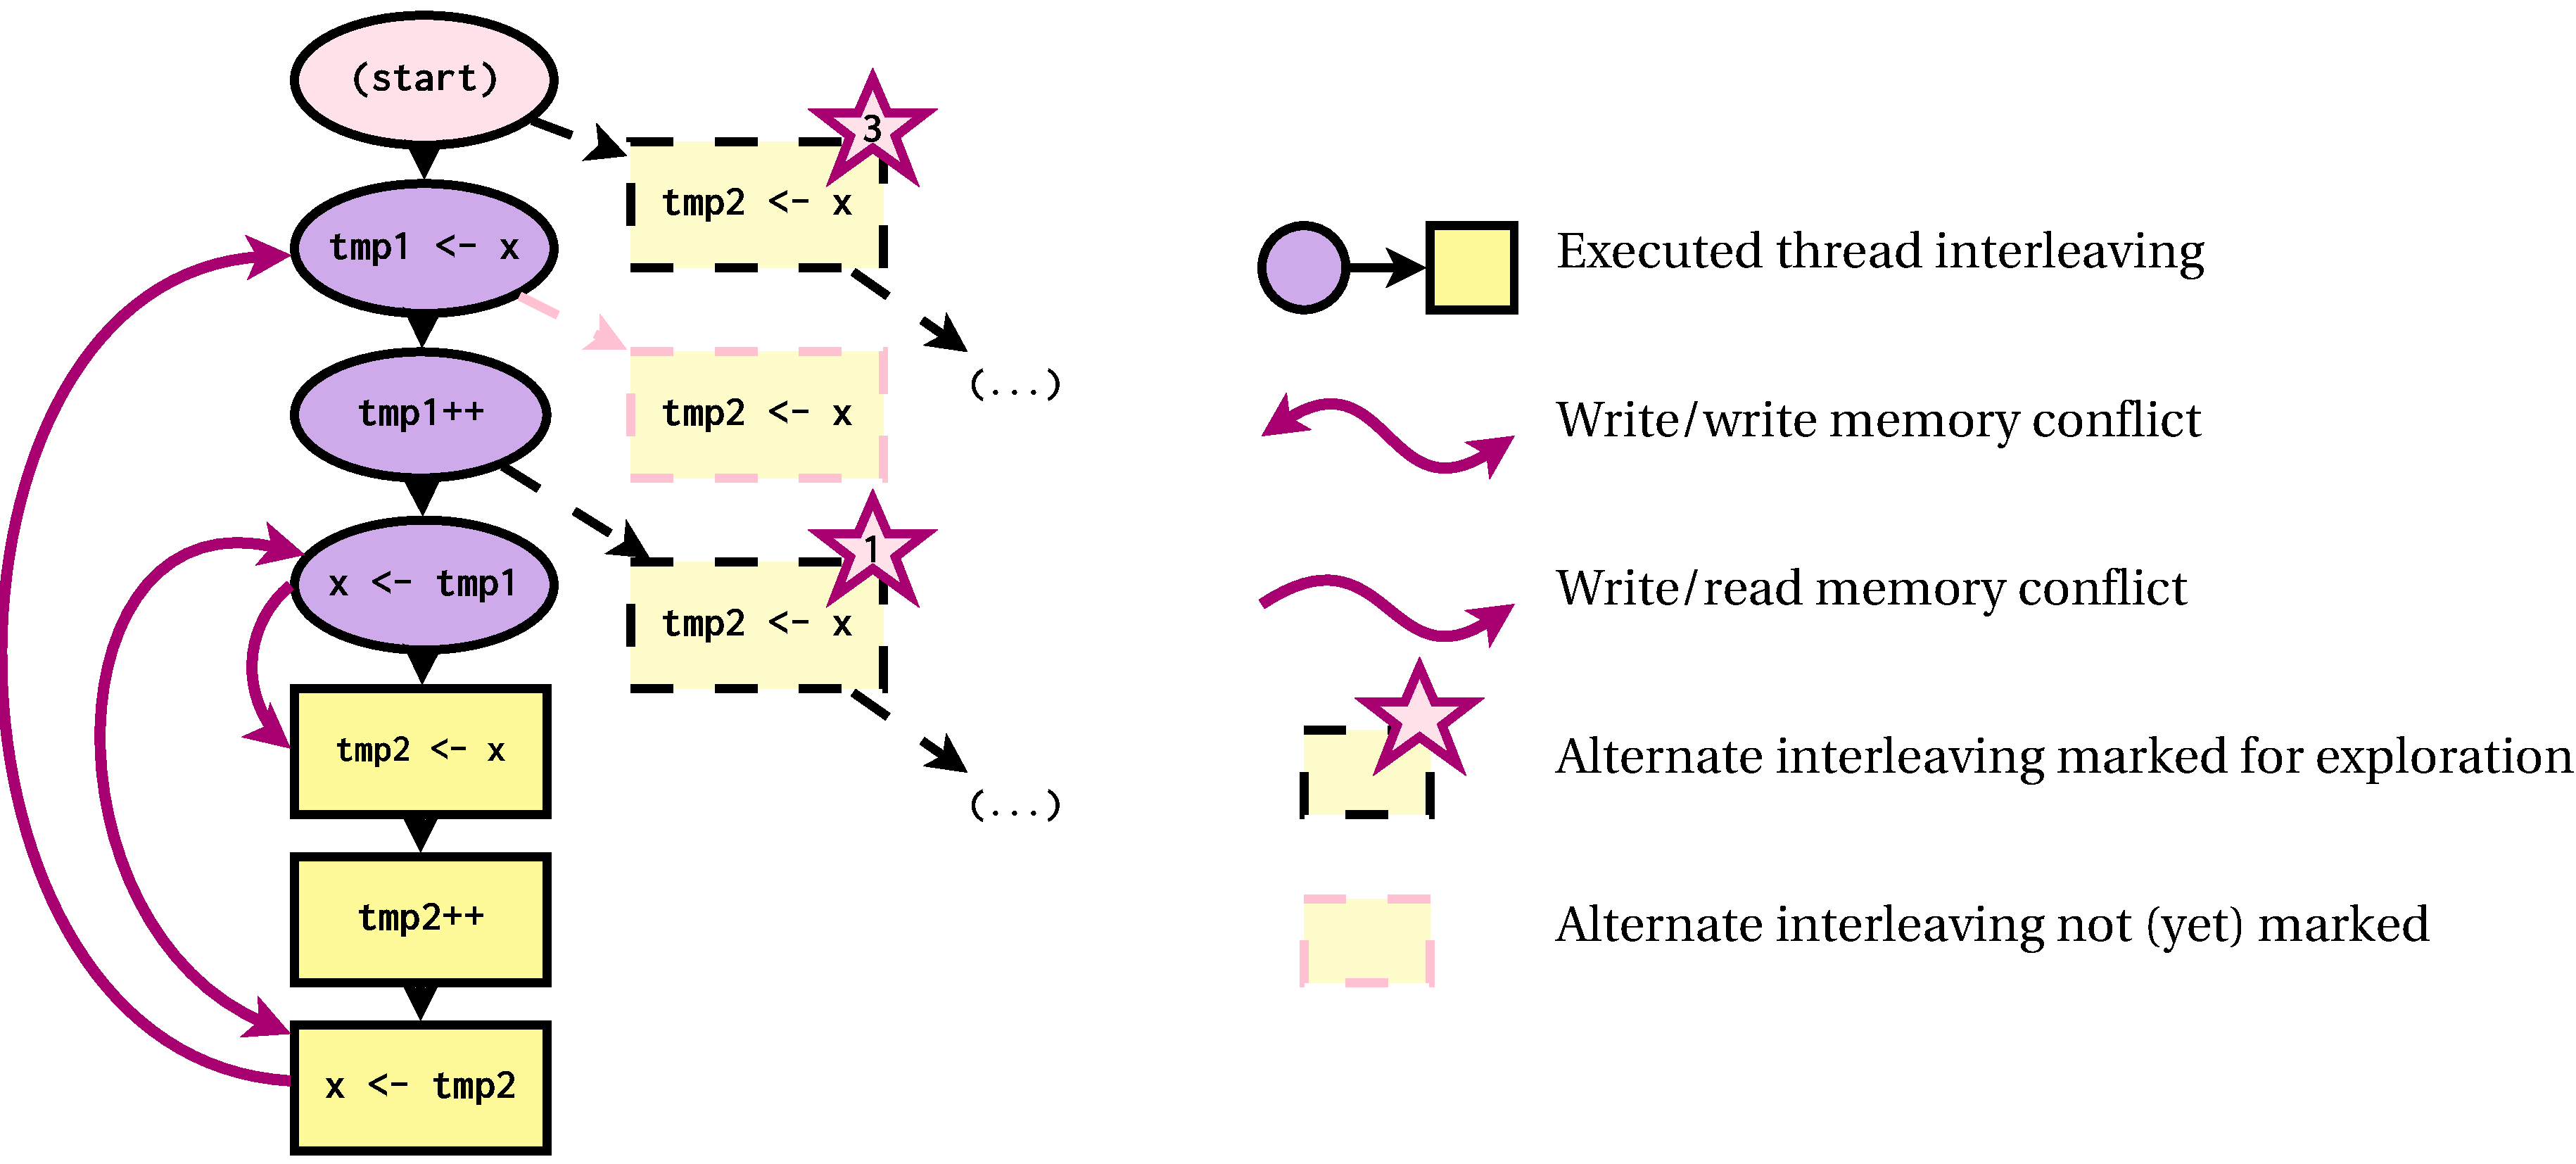
\includegraphics[width=\textwidth]{dpor-example-0.pdf}
	\end{center}
	\caption{Result of a single iteration of DPOR.}
	\label{fig:dpor-example-0}
\end{figure}

% trying to approximate the pastel background colors in something dark enough to render text in
\newcommand\dporTA[1]{\hilight{darklavender}{#1}\xspace}
\newcommand\dporTB[1]{\hilight{goldish}     {#1}\xspace}
\newcommand\dporTAcode[1]{\dporTA{\ensuremath{\mathbf{T_1}}: {\tt #1}}\xspace}
\newcommand\dporTBcode[1]{\dporTB{\ensuremath{\mathbf{T_2}}: {\tt #1}}\xspace}

In this interleaving, DPOR identifies 3 memory conflicts, two read/write and one write/write,
among the threads' 4 accesses to {\tt x}.
For each such pair, it ``marks'' an alternate interleaving,
which shall begin by preempting the thread of the first half of the conflict just before its execution thereof.
The ultimate goal is to execute an interleaving which reorders the conflict, which may expose new behaviour.
These marked interleavings form a work-queue which defines the exploration.
DPOR consumes from this set in depth-first order
(note the reversed order of $\bigstar$1 and $\bigstar$2)
to avoid storing in memory any representation of exponentially-sized subtrees outside of the current branch.
Note also that in $\bigstar$2,
the reordered \dporTB{{\tt tmp2~<-~x}} is not directly part of the memory conflict which marked it,
but it must be executed first to reach the conflicting \dporTB{{\tt x~<-~tmp2}}.

Now, let us run multiple iterations of DPOR
to advance through the first half of the full state space shown in \Cref{fig:tree}(b).
\Cref{fig:dpor-example-1} shows the outcome
(with the previously-marked $\bigstar$2, now re-labeled as $\bigstar$3, having its subtree abbreviated).

\begin{figure}[h]
	\begin{center}
		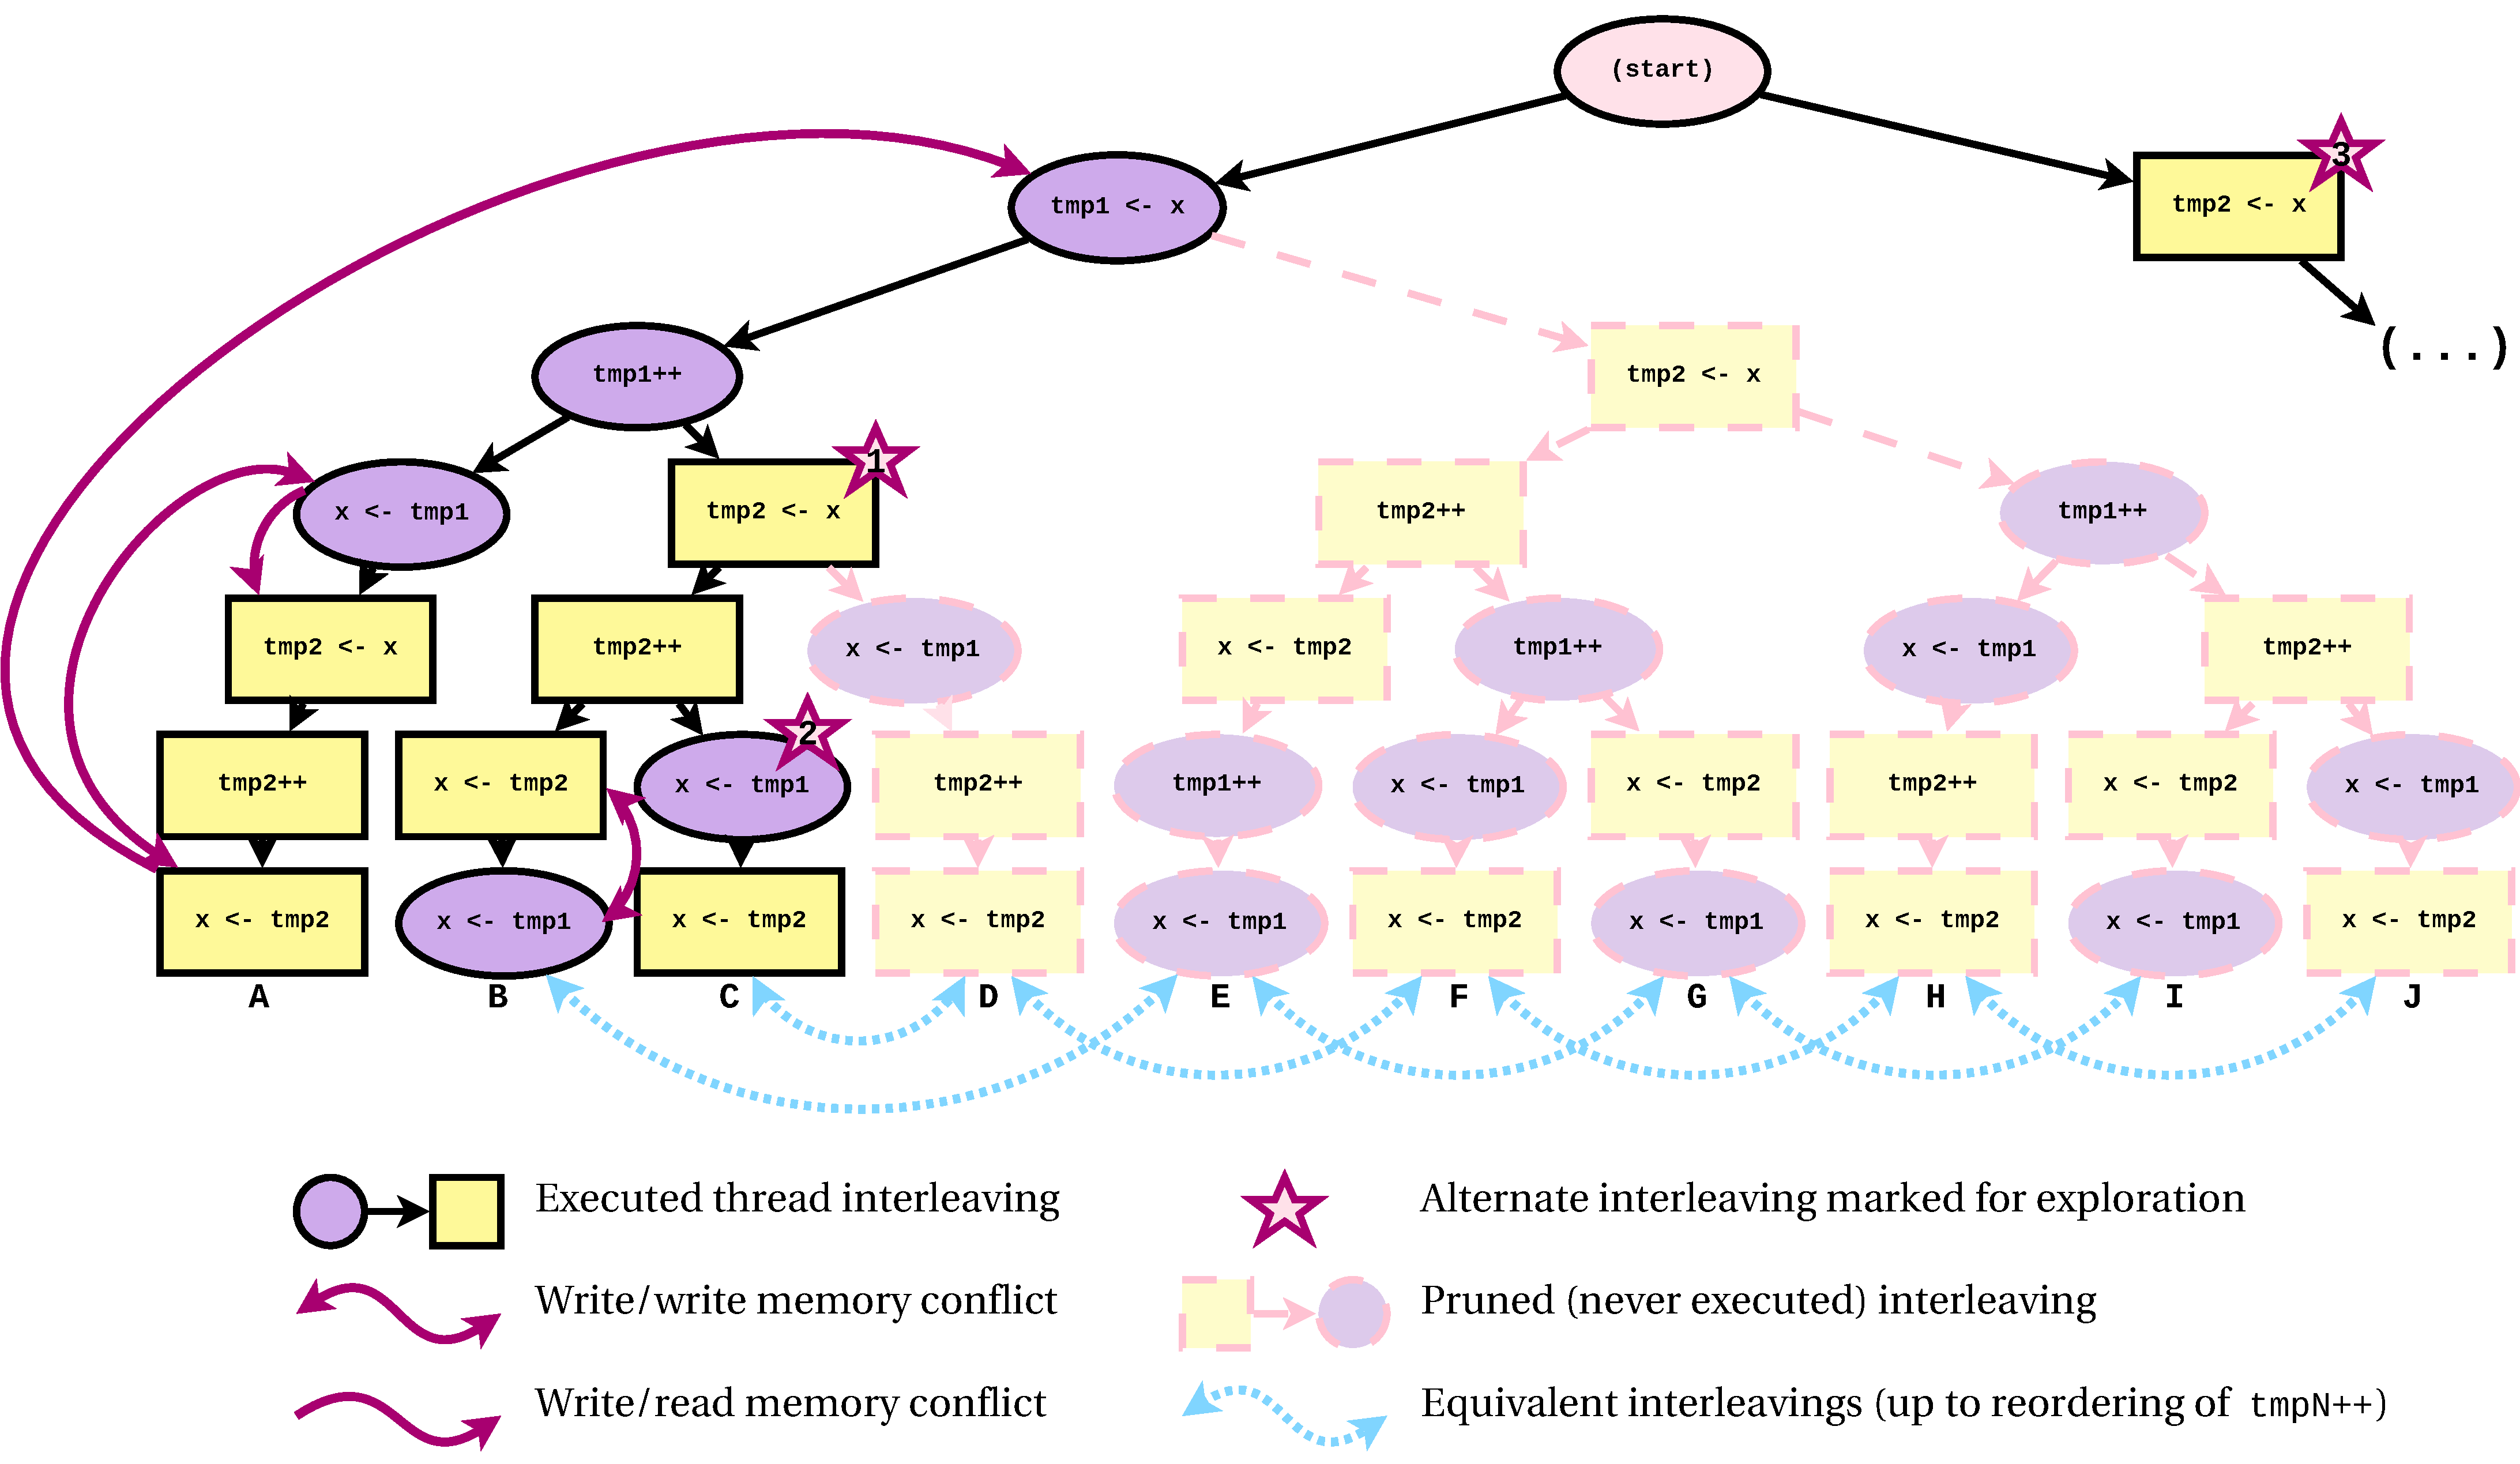
\includegraphics[width=\textwidth]{dpor-example-1.pdf}
	\end{center}
	\caption{Result of 3 DPOR iterations, pruning 7 redundant branches.}
	\label{fig:dpor-example-1}
\end{figure}

After marking $\bigstar$1 and $\bigstar$3 from \Cref{fig:dpor-example-0}'s interleaving, now labeled A,
DPOR advances to interleaving B, preferring to schedule the second thread before switching back to the first
to ensure the memory access is properly reordered.
From there, it identifies a new memory conflict, marks $\bigstar$2, and advances to C,
where it finds no memory conflicts that would mark anything not already marked and/or explored
(memory conflicts that were already reordered in old branches are not highlighted with arrows).
From C, $\bigstar$3 alone remains in the work-queue,
so DPOR advances to the second (symmetric) half of the state space,
skipping (thereby pruning) branches D through J.

To see why branches D through J need not be tested, consider that each thread's {\tt tmpN++} is a thread-local event,
participating in no memory conflicts,
and hence any two interleavings differing only by reordering {\tt tmpN++}s must be equivalent.
The dashed blue arrows denote such equivalences;
note the two disjoint equivalence classes \{B,E,G,I\} and \{C,D,F,H,J\},
distinguished by the order of the two final {\tt x~<-~tmpN}s.
Note also that
%(as shown in \Cref{fig:tree}(b)),
although B and C also have the same outcome ({\tt x==1}),
this depends on the {\em values} written to memory rather than {\em addresses}
(and would change if one thread's {\tt tmpN++} were a {\tt tmpN+=2}, for example),
which DPOR does not consider.
Recent work \cite{mcr} has extended DPOR to find such value-based equivalences,
although is beyond this explanation's scope.

Finally, let us consider the final result after DPOR runs out of remaining unexplored marked branches,
shown in \Cref{fig:dpor-example-2}.

\begin{figure}[h]
	\begin{center}
		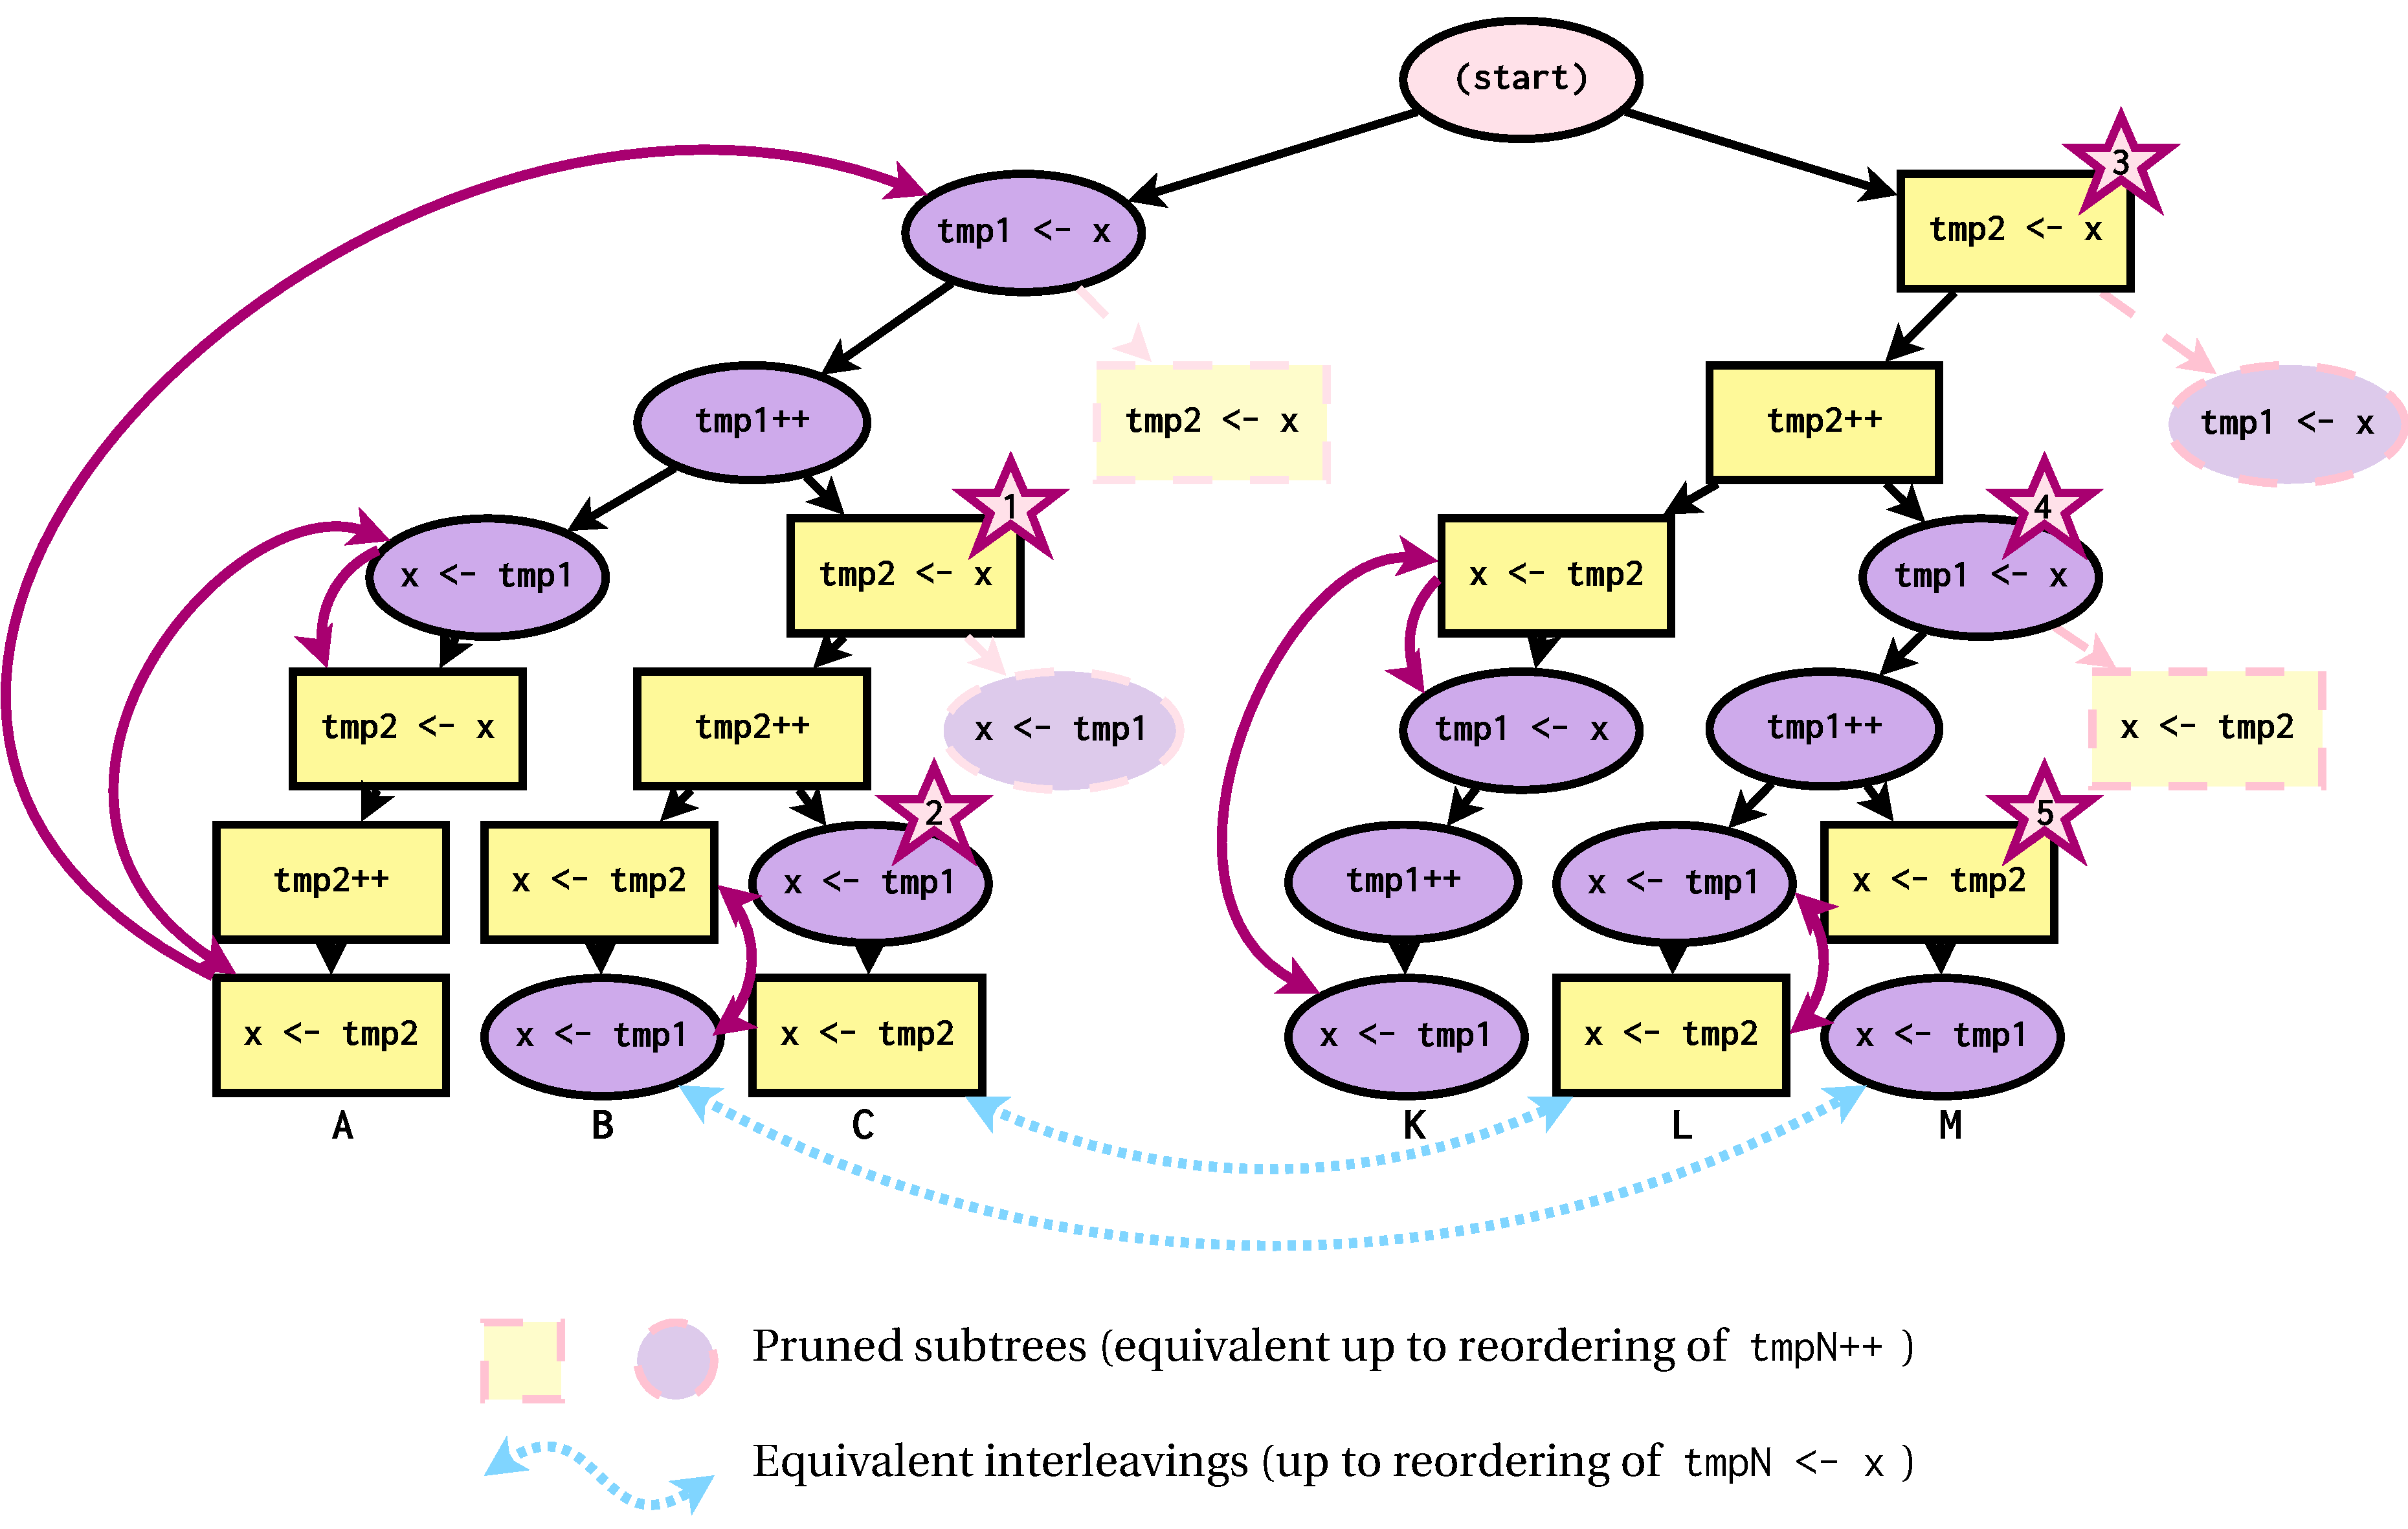
\includegraphics[width=\textwidth]{dpor-example-2.pdf}
	\end{center}
	\caption{DPOR's termination state, having reduced 20 interleavings to 6.}
	\label{fig:dpor-example-2}
\end{figure}

Ultimately, the second half of the state space is pruned symmetrically.
In general, the number of ways to interleave two threads executing $N$ and $M$ events each is given by ${N+M \choose N}$%
\footnote{Generalizing to $K$ threads, and simplifying to $N$ events each,
this formula becomes $\frac{n!k!}{n!^k}$.};
in this case, the original state space's size was ${3+3 \choose 3} = 20$.
DPOR's reduction is characterized by replacing $N$ and $M$ with the number of {\em conflicting} events only;
in this case, ignoring all {\tt tmpN++} reorderings and testing only ${2+2 \choose 2} = 6$ branches.

\subsubsection{Sleep set reduction}
\label{sec:landslide-sleepsets}

In the presence of non-conflicting transitions as well as conflicting ones,
DPOR's approach as described so far can still end up testing equivalent interleavings.
As the presence of more equivalence arrows in \Cref{fig:dpor-example-2} hints,
its reduced subset state space still contains redundancy,
arising from the fact that one pair of those \revisionminor{four} events is two reads, and hence not actually in conflict.
Visual inspection shows that $\bigstar$4, while locally justified
in trying to reorder \dporTA{{\tt tmp1~<-~x}} before \dporTB{{\tt x~<-~tmp2}},
effectively serves % oops
only to reorder it with \dporTB{{\tt tmp2~<-~x}}
relative to the first symmetric subtree ($\bigstar$1).
In other words,
even though DPOR marked each new branch with the intent only to reorder conflicting accesses,
$\bigstar$1 and $\bigstar$4 contained interleavings equivalent up to independent reorderings anyway.
\Cref{fig:sleepsets} summarizes the relevant interleavings to highlight one such equivalence.

\begin{figure}[h]
	\begin{center}
		\begin{tabular}{p{0.30\textwidth}p{0.30\textwidth}p{0.30\textwidth}}
	\begin{center}
	\begin{tabular}{l}
		\dporTAcode{tmp1 <- x (read)} \\
		\dporTBcode{tmp2 <- x (read)} \\
		\dporTAcode{x <- tmp1 (write)} \\
		\dporTBcode{x <- tmp2 (write)} \\
		% old example, pre dpor-example figure
		%$T_1$@$t_a$: \texttt{write~x} \\
		%$T_2$@$t_b$: \texttt{read~y} \\
		%$T_2$@$t_c$: \texttt{read~x} \\
	\end{tabular}
	\end{center}
	&
	\begin{center}
	\begin{tabular}{l}
		\dporTBcode{tmp2 <- x (read)} \\
		\dporTBcode{x <- tmp2 (write)} \\
		\dporTAcode{tmp1 <- x (read)} \\
		\dporTAcode{x <- tmp1 (write)} \\
		%$T_2$@$t_{b'}$: \texttt{read~y} \\
		%$T_2$@$t_{c'}$: \texttt{read~x} \\
		%$T_1$@$t_{a'}$: \texttt{write~x} \\
	\end{tabular}
	\end{center}
	&
	\begin{center}
	\begin{tabular}{l}
		\dporTBcode{tmp2 <- x (read)} \\
		\dporTAcode{tmp1 <- x (read)} \\
		\dporTAcode{x <- tmp1 (write)} \\
		\dporTBcode{x <- tmp2 (write)} \\
		%$T_2$@$t_{b'}$: \texttt{read~y} \\
		%$T_1$@$t_{a''}$: \texttt{write~x} \\
		%$T_2$@$t_{c''}$: \texttt{read~x} \\
	\end{tabular}
	\end{center}
	\\
	\begin{center}
	(a) Original branch (C).
	\end{center}
	&
	\begin{center}
	(b) Goal branch (K).
	\end{center}
	&
	\begin{center}
	(c) Redundant branch (L).
	\end{center}
	\end{tabular}
	\end{center}
	\caption[Motivating example for the sleep sets optimization.]
		{Motivating example for the sleep sets optimization.
	Three of \Cref{fig:dpor-example-2}'s interleavings are highlighted,
	with the always-independent {\tt tmpN++}s omitted for brevity.
	}
	\label{fig:sleepsets}
\end{figure}

Intuitively speaking,
when DPOR entered the $\bigstar$3 subtree,
it did not ``remember'' which memory conflict it wanted to reorder \dporTA{$\mathbf{T_1}$} around
(i.e., that \dporTB{{\tt x~<-~tmp2}} should come before \dporTA{{\tt tmp1~<-~x}}).
Upon witnessing the conflict in the new (intended) order,
it then tried to reorder it again,
producing interleavings regrettably equivalent to ones already tested
(all told, only \dporTB{{\tt tmp2~<-~x}} and \dporTB{{\tt tmp2++}} having been reordered around \dporTA{{\tt tmp1~<-~x}}).
%
To ``remember'' the original purpose of testing subtree $\bigstar$3,
which was already fulfilled by testing K,
DPOR can check just before tagging a new subtree (here, $\bigstar$4)
among all preceding transitions independent with the conflicting one
(here, \dporTB{{\tt tmp2~<-~x}} and \dporTB{{\tt tmp2++}} independent with \dporTA{{\tt tmp1~<-~x}})
for an already-explored interleaving beginning with the target thread.
%(here, the original sibling of $\bigstar 3$).
If such exists,
the new subtree is guaranteed to be equivalent to one already checked,
and can safely be skipped.

Landslide implements this check in {\tt equiv\_already\_explored()},
which checks (in this case after executing K),
that if the first event to be reordered (here, \dporTA{{\tt tmp1~<-~x}})
has already been tested in an equivalent reordering around any number of preceding events
(here, \dporTB{{\tt tmp2~<-~x}} and \dporTB{{\tt tmp2++}}),
then the newly marked subtree is safe to prune.
Note that this does not require storing any full subtrees outside of the current branch;
only the subtree's root node need be saved to
prove that an equivalent interleaving beginning with \dporTA{$\mathbf{T_1}$} therein was already checked,
preserving DPOR's $O(n)$ memory footprint.

This corresponds to the {\em sleep sets} optimization described by prior work \cite{partial-order-methods,dpor,optimal-dpor},
so named because it effectively puts \dporTA{$\mathbf{T_1}$}
``to sleep'' until after the true conflicting access of \dporTB{{\tt x~<-~tmp2}}.
Landslide's implementation differs from prior work,
which explicitly tracks sets of reordered threads and expected conflicting accesses,
by instead identifying
where the reduction should occur
during subsequent DPOR iterations.
% KEEP_RUNNING_DPORS_CHOSEN_TID
This approach also relies on the search ordering strategy ({\tt arbiter\_choose()})
to prefer scheduling the thread previously chosen for reordering by DPOR,
to ensure the conflicting access happens before the preempted thread gets a chance to run again.
%to force whatever its conflicting memory access was to happen before the other, preempted thread gets a chance to run.
Further optimizations such as {\em source sets} and {\em wakeup trees},
which prior work has shown achieve optimality
(i.e., executing exactly one interleaving per equivalence class) \cite{optimal-dpor}
are not yet implemented.
To the best of my knowledge,
they provide further reduction only in cases of 3 or more threads;
I suspect (without proof) that sleep-set DPOR is optimal for 2 threads.

\Cref{chap:quicksand}'s experiments and \Cref{chap:education}'s user studies
were conducted before this optimization was implemented.
Note that its absence has no bearing on DPOR's soundness, only its efficiency,
and that Landslide showed good bug-finding performance even without it.
\Cref{chap:tm}'s experiments include this optimization,
because its presence was required to fairly compare the other reduction strategies presented therein.

%%%%%%%%%%%%%%%%%%%%%%%%%%%%%%%%%%%%%%%%%%%%%%%%%%%%%%%%%%%%%%%%%%%%%%%%%%%%%%%%

\subsection{State space estimation}
\label{sec:landslide-estimate}

For both the user's convenience and for Quicksand's prioritization algorithm (\cref{sec:quicksand-id}),
Landslide attempts to guess how big partially-explored state spaces will ultimately end up being upon completion.
Because the backtracking implementation uses checkpointing
rather than replaying similar interleavings' shared execution prefixes from the beginning \cref{sec:landslide-timetravel},
the total number of interleavings (i.e., leaf nodes in the execution tree)
must be estimated separately from the total runtime (i.e., sum of all edge weights in the tree).

As a concrete example, consider the state space of \Cref{fig:dpor-example-2},
and suppose each transition to the next preemption point takes 1 second to execute.
While the first branch executes in 6 seconds,
the second branch, sharing the first transition as a common prefix, takes 4 seconds,
and the one after that only 2;
the state space being ultimately completed in 24 seconds.
Even with perfect hindsight,
na\"ively multiplying the total interleavings (6)
by the total execution time per branch (6) would double-count common prefixes
and grossly overestimate (36) the total runtime.

Hence, Landslide uses two differently suitable algorithms for each of size and runtime estimation:
the Weighted Backtrack Estimator (WBE) and the Recursive Estimator (RE), respectively,
first introduced in \cite{estimating-search-tree-size} and later adapted to DPOR by \cite{estimation}.
In principle, both calculate the current progress as a proportion of the expected total
by counting how many branches DPOR has marked for future exploration (\cref{sec:landslide-explore})
and assuming the sizes of their resulting subtrees are predicted by the known sizes of similar already-explored subtrees.
In practice, the calculation strategy differs between the two approaches,
which can occasionally result in drastically differing outputs (\cref{sec:tm-verif}).

Implementation-wise, Landslide reports size estimates as both the percentage and as a total number of branches,
and time estimates as an ETA.
Quicksand's {\tt -v} option (\cref{sec:landslide-quicksand-options})
will cause it to print them each time a new interleaving is tested; for example:
\begin{center}
	{\tt \small [JOB 1] progress: 66101/94825 brs (69.708252\%), ETA 13m 37s (elapsed 46m 10s)}
\end{center}
Both estimates are computed simultaneously in {\tt \_estimate()} in {\tt estimate.c}
(which, I might add, is well-commented in case the following prose is insufficient).
%I summarize their respective implementations here.
\Cref{chap:warpzone-heuristics} will discuss their limitations and some opportunities for future improvement.

\subsubsection{Size (Weighted Backtrack) estimation}

The WBE, used to estimate total number of interleavings,
computes the {\em proportion} of the total size
that the already-explored branches are expected to comprise,
using DPOR's workqueue to anticipate how many unexplored marked branches remain.
This serves as a progress bar \cite{progress-bar} that represents the estimated percentage towards completion,
approaching 100\% (not necessarily monotonically) as exploration continues.

Summarizing prior work's formal definition \cite{estimation},
the proportion at a terminal node $v_n$%
\footnote{Prior work \cite{estimating-search-tree-size,estimation} refers to this instead as {\em probability},
i.e., the probability that the node will appear in a branch chosen uniformly at random from the completed tree.
I find ``proportion'' to be more illuminating on how the algorithm works.
},
preceded by an execution sequence $(v_1 \dots v_{n-1})$,
is computed as:%
\footnote{
Simplified from \cite{estimation}: the missing $F(v_i)$ is 0, using the empty fit strategy.
}

\[
	\mathsf{proportion}(v_1 \dots v_n) = \displaystyle\prod_{i=1}^{n-1} \frac{1}{|\mathsf{marked~children}(v_i)|}
\]

where $\mathsf{marked~children}(v_i)$ is the number of enabled thread transitions at $v_i$
which have either already been explored or been marked by DPOR.
Then, the total estimate is given as the sum over all branches $b = (v_1 \dots v_n)$ explored so far:%
\footnote{
Simplified from \cite{estimation}: $t(b)$, the time for each branch, is 1, because we are counting them.
}

\[
	\mathsf{estimate} = \frac{1}{\sum_{b \in B} \mathsf{proportion}(b)}
\]

It is easy to see how these might fit into DPOR's incremental search procedure:
at the end of each branch compute its $\mathsf{proportion}$ and add it in to a global $\mathsf{estimate}$ value.
However, DPOR may tag new branches to explore that would affect past branches' proportions,
requiring them to be recomputed,
%which is not feasible without
which would require
storing the entire exponentially-sized tree in memory.
Instead, Landslide also stores per-subtree estimates at intermediate $v_i$ nodes, $1 < i < n$,
along the current branch.
Whenever DPOR marks a new $k$th branch
%for exploration
at some $v_i$
%with $\mathsf{marked~children}(v_i) = k$,
its estimate
is multiplied by $(k-1)/k$ to retroactively adjust all past branches' proportions contributing to that estimate.
The change is also propagated to its sub-subtrees,
whose estimates must also incorporate the new $\mathsf{marked~children}$ value.
This allows Landslide to update the global estimate after each branch in $O(n)$ time and memory,
without recomputing past branch proportions individually.

\subsubsection{Run-time (Recursive) estimation}

The RE, used to estimate total execution time,
computes at each node the expected time to execute all subtrees rooted at children of that node,
assuming unvisited subtrees' times will be an average of their visited siblings.
This estimate at the root node, minus the current time elapsed so far,
serves as a guess at how long until completion.
Let $\mathsf{usecs}(v_i)$ denote the time elapsed during execution of the transition $v_{i-1} \rightarrow v_i$.
Then a node's estimate is given by:

\[
	\mathsf{estimate}(v_i) = \mathsf{usecs}(v_i) +
	\frac{|\mathsf{marked~children}(v_i)|}{|\mathsf{explored~children}(v_i)|}
	\sum_{v_j \in \mathsf{explored~children}(v_i)} \mathsf{estimate}(v_j)
\]

Like the WBE, whenever DPOR tags a new $k$th child at some $v_i$,
its estimate is multiplied by $k/(k-1)$ (note the reciprocal of before)
to retroactively re-weight previously explored subtrees' estimates.
Unlike the WBE, this change does not need to be propagated to descendant subtrees' estimates.
This estimate also takes $O(n)$ time and memory.

\subsubsection{Example}

To illustrate how the two estimators can under-estimate the total tree size and/or diverge from each other,
consider the state space from \Cref{fig:dpor-example-2}, of size 6.
Suppose for RE that each transition takes 1 second to execute.

\begin{enumerate}
	\item After branch A, two tags exist, $\bigstar$1 and $\bigstar$3.
		Under WBE, the subtree estimate at \dporTA{{\tt tmp1++}} will first be 1/2
		(half its children being fully explored),
		and the root estimate will be 1/4,
		half that,
		which is propagated back down to \dporTA{{\tt tmp1++}}, becoming also 1/4.
		Dividing the current progress (1) by that yields 4 total branches, an underestimate.

		Under RE, the estimate at \dporTA{{\tt tmp1++}} will be 9 seconds
		(incorrectly assuming $\bigstar$1's subtree will be 1 branch),
		and the root estimate will be 20 seconds, an underestimate.
	\item After branch B, $\bigstar$2 is now marked.
		Under WBE, the subtree estimate at \dporTB{{\tt tmp2++}} is 1/2,
		which at \dporTA{{\tt tmp1++}} is then divided by its $\mathsf{marked~children}$
		and added to its estimate, yielding 3/4.
		Note that it has ``forgotten'' that only branch A, alone, contributed to its original 1/2,
		rather than two branches as in this subtree.
		The root and \dporTA{{\tt tmp1++}}'s subtree estimates are updated (and propagated down) to 3/8.
		Dividing the current progress (2) by that yields 5.33 branches, an underestimate.

		Under RE, the estimate at \dporTB{{\tt tmp2++}} is 5 seconds,
		the estimate at \dporTA{{\tt tmp1++}} is updated to 11 seconds,
		and the root estimate to 24 seconds, accurate.
	\item After branch C, nothing new was marked.
		The subtree estimate at \dporTB{{\tt tmp2++}} is 1
		(having been completely explored)
		and the root estimate is 1/2.
		Dividing the current progress (3) by that yields 6, accurate.

		Under RE, no estimates change from after B.
	\item After branch K, $\bigstar$4 now exists.
		\dporTB{{\tt tmp2++}}'s subtree estimate is at first 1/2,
		then the root estimate and it get updated to 3/4.
		Dividing into the current progress (4), 5.33, an underestimate.

		Under RE, the estimate at \dporTB{{\tt tmp2++}} is 9 seconds,
		and the root estimate is 22 seconds, an underestimate.
	\item After branch L, $\bigstar$5 joins the party.
		\dporTB{{\tt tmp2++}}'s estimate is updated to 3/4,
		and the root estimate ultimately becomes 7/8.
		Dividing into the current progress (5), 5.7, an underestimate.

		Under RE, the estimate at \dporTB{{\tt tmp2++}} is 11 seconds,
		and the root estimate is 24 seconds, accurate.
	\item After branch M, both estimators have perfect information and converge to accuracy.
\end{enumerate}

To illustrate how the estimators can over-estimate the total tree size,
consider the same state space,
except with the $\bigstar$4 subtree also pruned by DPOR's sleep sets extension (\cref{sec:landslide-sleepsets});
i.e., only branches A, B, C, and K remain,
with an 18 second execution time.
Both estimators' behaviour is identical through branch C,
only now WBE's prediction happens to be accurate at A (although for the wrong reasons),
but overestimates at B and C,
while RE's predictions are all overestimates.
As before, both reach perfect accuracy upon completion, now occurring at K.
Intuitively speaking, the estimators underpredict when DPOR keeps finding new branches to tag as it makes progress,
and overpredict when sleep set reduction achieves extra pruning on right subtrees.
Not shown in this example, interleaving-dependent control flow can, of course,
beget unexpected state space structure in essentially arbitrary other ways.

%%%%%%%%%%%%%%%%%%%%%%%%%%%%%%%%%%%%%%%%%%%%%%%%%%%%%%%%%%%%%%%%%%%%%%%%%%%%%%%%

\subsection{Data race analysis}
\label{sec:landslide-datarace}

Whenever a memory conflict is identified for DPOR as described above,
the access pair's corresponding locksets and/or happens-before edges are checked to determine if it's also a data race.
Note the distinction: DPOR memory conflicts indicate that two thread transitions,
if reordered, could produce different behaviour, even if all accesses therein are adequately synchronized;
while a data race indicates furthermore that the two threads can be interleaved precisely at the moment of one or both accesses,
supposing that a new preemption point were introduced to split one or both transitions in half.
% nb. i think "only one of the accesses can be preempted at and have the other interleaved inside, but not the other way around,
% is a property of cli/sti involvement in kernel space only.

The core of the comparison is in {\tt check\_locksets()} in {\tt memory.c}.
It checks each DPOR memory conflict's locksets, for limited happens-before,
and happens-before edges, for pure happens-before
(\cref{sec:background-hb}).

\subsubsection{Limited Happens-Before}
\label{sec:landslide-lhb}

Conditions \#1, \#2, and \#4 defined in \cref{sec:background-hb},
provided the Limited Happens-Before definition for \#4,
coincide with DPOR's version of happens-before described in the previous section.
%coincide exactly with the conditions to be considered a memory conflict under DPOR.
Hence all that remains to be checked is \#3, the set of locks held by each thread at the time of access.

Routines for recording lockset changes and computing set intersection are found in {\tt lockset.c}.
Apart from standard data structure manipulation,
one algorithmic point of note is that locks are distinguished by types in addition to address.
This allows (e.g.) mutexes stored as part of the implementation of semaphores to protect a different set of accesses than are protected by the semaphore they implement.

% TODO: talk abt free re malloc false positives

\subsubsection{Pure Happens-Before}
\label{sec:landslide-phb}

In Pure Happens-Before,
condition \#4 is replaced with the traditional distributed systems notion of Happens-Before \cite{lamport-clocks}.
Landslide implements this via the vector clocks approach described by {\sc FastTrack} \cite{fasttrack}.
I refer the reader interested in the vector clock algorithm itself to the {\sc FastTrack} paper,
limiting discussion here to Landslide's corresponding implementation of each inference rule.

I use the \revisionminor{{\sc Djit+} rules \cite{djit} (as presented in \cite{fasttrack})}
for reads and writes rather than the {\sc FastTrack} ones,
even though they more often incur $O(n)$ runtime in the size of the vector clocks:
because Landslide tests should be limited to few threads in order to manage the state space size,
$n$ is always in the single digits, so I optimize for code simplicity.

\begin{itemize}
	\item Reads and writes ({\tt memory.c})
	\begin{itemize}
		\item \textsc{Djit+ read/write same epoch} - {\tt vc\_eq()} case of {\tt add\_lockset\_to\_shm()}
		\item \textsc{Djit+ read/write} - {\tt vc\_happens\_before()} case of {\tt check\_locksets()}
	\end{itemize}
	\item Synchronization ({\tt schedule.c})
	\begin{itemize}
		\item \textsc{FT acquire}
			\begin{itemize}
				\item {\tt kern\_mutex\_\{,try\}locking\_done()} cases of {\tt kern\_update\_state\_\allowbreak{}machine()}
				\item {\tt user\_mutex\_\{,try\}lock\_exiting()} cases of {\tt user\_update\_state\_\allowbreak{}machine()}
				\item {\tt cli} case of {\tt kern\_update\_state\_machine()} (Pintos only)
				\item {\tt cli}/{\tt sti} lock handoff case in {\tt sched\_update()} (Pebbles only)
			\end{itemize}
		\item \textsc{FT release}
			\begin{itemize}
				\item {\tt kern\_mutex\_unlocking()} case of {\tt kern\_update\_state\_machine()}
				\item {\tt user\_mutex\_unlock\_entering()} case of {\tt user\_update\_state\_machine()}
				\item {\tt sti} case of {\tt kern\_update\_state\_machine()} (Pintos only)
				\item {\tt cli}/{\tt sti} lock handoff case in {\tt sched\_update()} (Pebbles only)
			\end{itemize}
		\item \textsc{FT fork} - {\tt agent\_fork()}
		\item \textsc{FT join} - {\tt sched\_unblock()} case of {\tt kern\_update\_state\_machine()}
			(Pebbles only; Pintos case is handled by above {\tt cli}/{\tt sti} cases in context switch)
	\end{itemize}
\end{itemize}

%%%%%%%%%%%%%%%%%%%%%%%%%%%%%%%%%%%%%%%%%%%%%%%%%%%%%%%%%%%%%%%%%%%%%%%%%%%%%%%%

\subsection{Iterative Context Bounding}
\label{sec:landslide-icb}

Iterative Context Bounding \cite{chess-icb} is a state space exploration strategy
that prioritizes interleavings with fewer total preemptions first.
Let $P(S)$ denote the number of preemptions in an execution sequence $S$.
Then, to summarize in pseudocode a na\"ive exploration of some state space $U$ as:

\begin{algorithm}[h]
	\ForEach{$S \in U$}{
		Execute($S$)
	}
	\caption{Straightforward exploration ordering.}
	\label{alg:not-icb}
\end{algorithm}

% TODO: make sure latex doesn't fuck up the algorithm placement
ICB's approach could likewise be summarized as follows:

\begin{algorithm}[h]
	\For{$B \in [0..\mathsf{max}_P(U)]$}{
		\ForEach{$S \in U, P(S) \le B$}{
			Execute($S$)
		}
	}
	\caption{ICB exploration ordering.}
	\label{alg:icb}
\end{algorithm}

%% stupid imperative way to write it
%\begin{algorithm}[h]
%	\For{$B \in [0..\infty]$}{
%		$\mathsf{skipped\_any} := \mathsf{false}$ \\
%		\ForEach{$S \in U$}{
%			\uIf{$P(S) \le B$}{
%				Execute($S$)
%			} \Else {
%				$\mathsf{skipped\_any} := \mathsf{true}$
%			}
%		}
%		\If{$\neg \mathsf{skipped\_any}$}{
%			{\bf Break}
%		}
%	}
%\end{algorithm}

\subsubsection{Implementation}

First of all, note that \Cref{alg:icb} is structured in a way that repeats interleavings
with fewer than $n$ preemptions that have already been checked in previous iterations of the outer loop.
This is because the number of preemptions in each branch is not known in advance;
rather, the state space must always be explored in an overall depth-first approach,
at best skipping too-preemptful interleavings as they are encountered.
As simple as it would be to state ``{\bf foreach} $S \in {\mathsf{sort}_P(U)}$'' in pseudocode,
implementing such an ordering would be much less straightforward. %
% TODO: post committee review
%\footnote{Translating conference papers' pseudocode into usable implementations is often quite difficult \cite{itg2}.}

Therefore, Landslide's ICB implementation combines with DPOR
when tagging new branches to explore at the end of each branch:
just as DPOR skips alternate interleavings that are memory-independent,
ICB further filters interleavings requiring more preemptions than the current bound
out of the to-explore set.
The macro {\tt ICB\_BLOCKED},
defined in {\tt schedule.h},
decides if a given thread would require a preemption beyond the current bound to switch to.%
\footnote{Since ``voluntary'' context switches (e.g. arising from {\tt yield()})
are often necessary for correct execution,
{\tt ICB\_BLOCKED} does not count such switches towards the preemption count.
Therefore, within a certain preemption bound $B$,
interleavings with more than $B$ context switches may still be tested.
}
The DPOR implementation then checks, for some $I_{ij}$ it wants to mark for exploration,
whether {\tt ICB\_BLOCKED}($T_j$) at the state after $t_i$,
and skips it if so ({\tt tag\_good\_sibling()}/{\tt tag\_all\_siblings()}).

Then, the entire state space is repeated with increasing bound until no such are filtered.
This core ICB loop appears in {\tt time\_travel()} in {\tt landslide.c}.
Although not explicitly structured as a C-style loop in the code,
it resets Landslide's progress through the state space,
allowing exploration to continue until it finally observes all interleavings to have fewer preemptions than the bound.

\subsubsection{Complexity}

If the search is terminated early after reaching a predetermined fixed bound for $B$,
ICB in principle reduces the state space from exponentially-sized%
\footnote{Combinatorial, to be precise; see \cref{sec:landslide-dpor-example}.}
in both $K$, the number of threads,
and $N$, the number of events,
to still exponential in $K$ (typically small) but only polynomial in $N$ (typically large).
Under a preemption bound of $B$, there are only $B+K$ opportunities for context switching%
\footnote{This $K$ appears from the ``mandatory'' context switches at thread exit;
more of which could also be introduced from blocking synchronization.},
% "roughly" - i.e., this formulation allows choosing all B preemptions from the same thread,
% which is only possible when K >= B i guess
% it's an overapproximation but getting it more precise seems like it'd be way more complex,
% and the overapproximation is good enough to make this point anyway
% also an underapprox because this doesn't count interleavings with b<B preemptions but that's a constant factor
so the corresponding state space size is at most ${KN \choose B}(B+K)!$.
All $N$-related factors therein are bounded above by $N^B$.

Prior work often recommends 2 for such a cutoff \cite{chess-icb,smc-empirical-study,dejafu},
although \cref{sec:quicksand-eval}'s larger dataset suggests 3 would be considerably more thorough.
On the other hand, any finite such bound can provide only a heuristic verification guarantee. %anymore.
Preserving the full formal verification, i.e., continuing iteration until $B = \mathsf{max}_P(U)$
not only remains exponential in $N$,
% again overapproximating because each previous iteration is combinatorially smaller than the next
but also introduces a factor of $\mathsf{max}_P(U)$ repeated work.
\revisionminor{Landslide takes this approach for now (rather than stopping at any finite cutoff).}
Future work could memoize already-tested interleavings so that each iteration of $B$ could test only
those schedules with exactly $B$ preemptions,
restoring the original $B$-independent (but still exponential) complexity.

\subsubsection{Bounded Partial-Order Reduction}

Prior work \cite{bpor} has shown that
when combined with DPOR to prune equivalent interleavings,
DPOR's reduction might not be sound with respect to the subset of $U$ under $P \le n$.
That work introduced Bounded Partial Order Reduction (BPOR),
a compatibility extension to DPOR for ICB to address this problem.

To summarize, when DPOR identifies some interleaving $I_{ij}$ to test,
it may not be possible to execute $T(t_j)$ after $t_i$ without exceeding the current preemption bound.
However, there may exist another interleaving $J_{i'j}$ within the bound which runs $T(t_j)$ before $t_i$.
If a DPOR implementation na\"ively configured with ICB simply skipped $I$ on account of the preemption bound,
$J$ may not get marked for exploration
from any other iteration and/or pair of conflicting transitions.
Even though restricting the state space to a certain maximum preemption bound is already unsound
in terms of losing full interleaving coverage,
failing to test even $J$ would be a failure of DPOR itself
to soundly prune the already-reduced state space defined by that bound.
Hence the need for BPOR, to ensure that if such an alternative $J$ to $I$ exists within the bound,
it gets marked for exploration immediately.

To implement BPOR,
whenever {\tt ICB\_BLOCKED} causes DPOR to skip an interleaving,
Landslide searches all transitions $t_k \in S$
such that $t_k \prec_S t_i$ and $T(t_k) = T(t_i)$ and
$\neg$\{$\exists t_l \in S$ such that $t_k \preceq_S t_l \prec_S t_i$ and $T(t_l) = T_j$\}
({\tt stop\_bpor\_backtracking()}).
All $I_{kj}$s which can be tested within the preemption bound are marked instead of $I_{ij}$
({\tt tag\_reachable\_aunts()}).
The reader interested in further algorithm details and the corresponding soundness proof is referred to \cite{bpor}.

%%%%%%%%%%%%%%%%%%%%%%%%%%%%%%%%%%%%%%%%%%%%%%%%%%%%%%%%%%%%%%%%%%%%%%%%%%%%%%%%

\subsection{Heuristic loop, synchronization, and deadlock detection}
\label{sec:landslide-blocking}

Despite the ease of automatically instrumenting a fixed concurrency API such as P2's,
the variety of student implementations inevitably results in many behaviours outside Landslide's model.
This section documents the heuristics Landslide uses to approximate a program's formal behaviour in such situations.

\subsubsection{Infinite loop detection}

All modern presentations of stateless model checking assume finite program length.
Even though all test cases used in this thesis's experiments are hand-written to ensure runtime
\revisionminor{which is}
not just finite but also short (on account of exponential state space sizes),
bugs may still cause a program to get stuck in an infinite loop unexpectedly.
Detecting such loops in general is of course uncomputable \cite{entscheidungsproblem},
but Landslide has the benefit of knowledge from past iterations to inform its sense of how long the program ``should'' run.

\begin{figure}[h]
	\begin{center}
		\begin{tabular}{cc}
			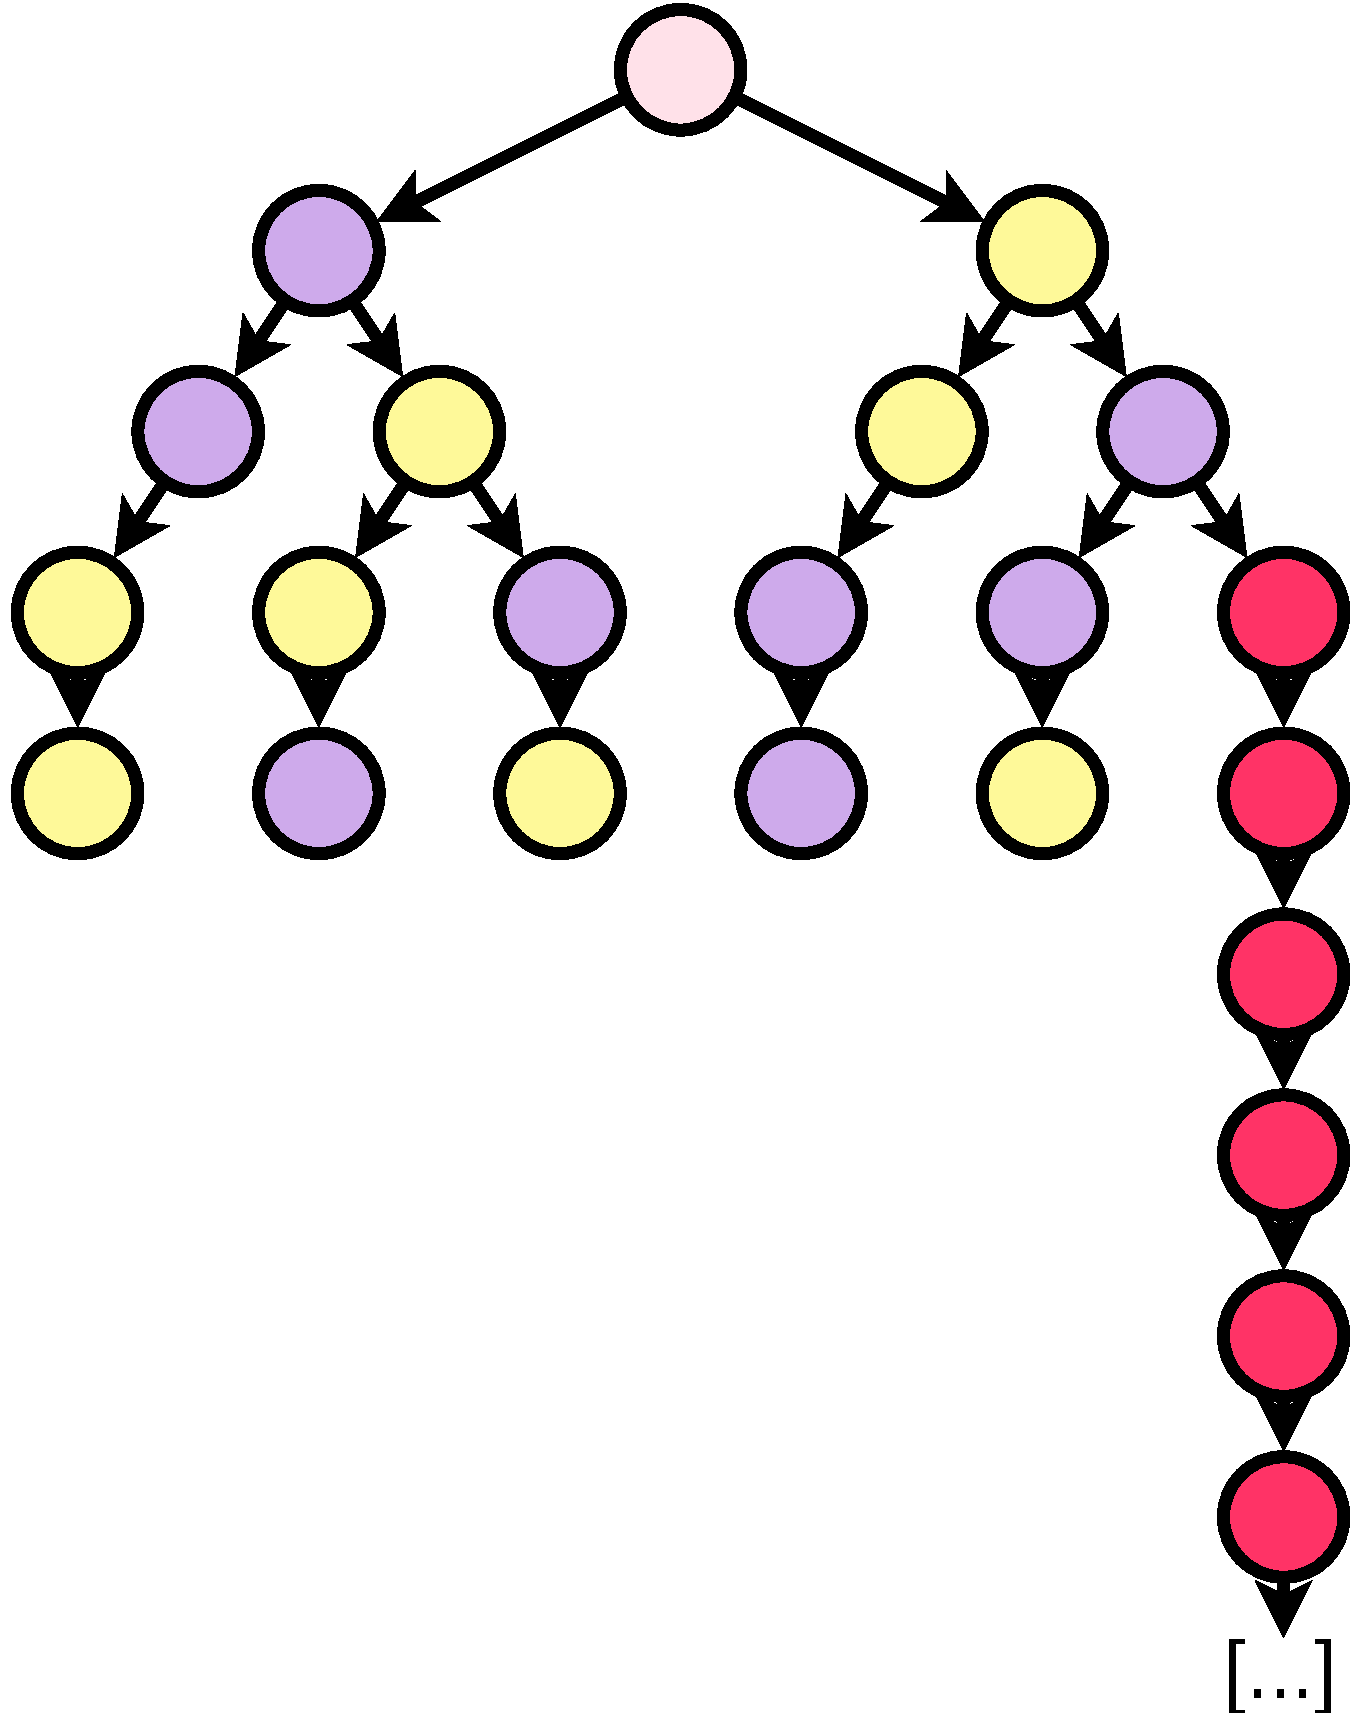
\includegraphics[width=0.28\textwidth]{heuristic-livelock.pdf}
			&
			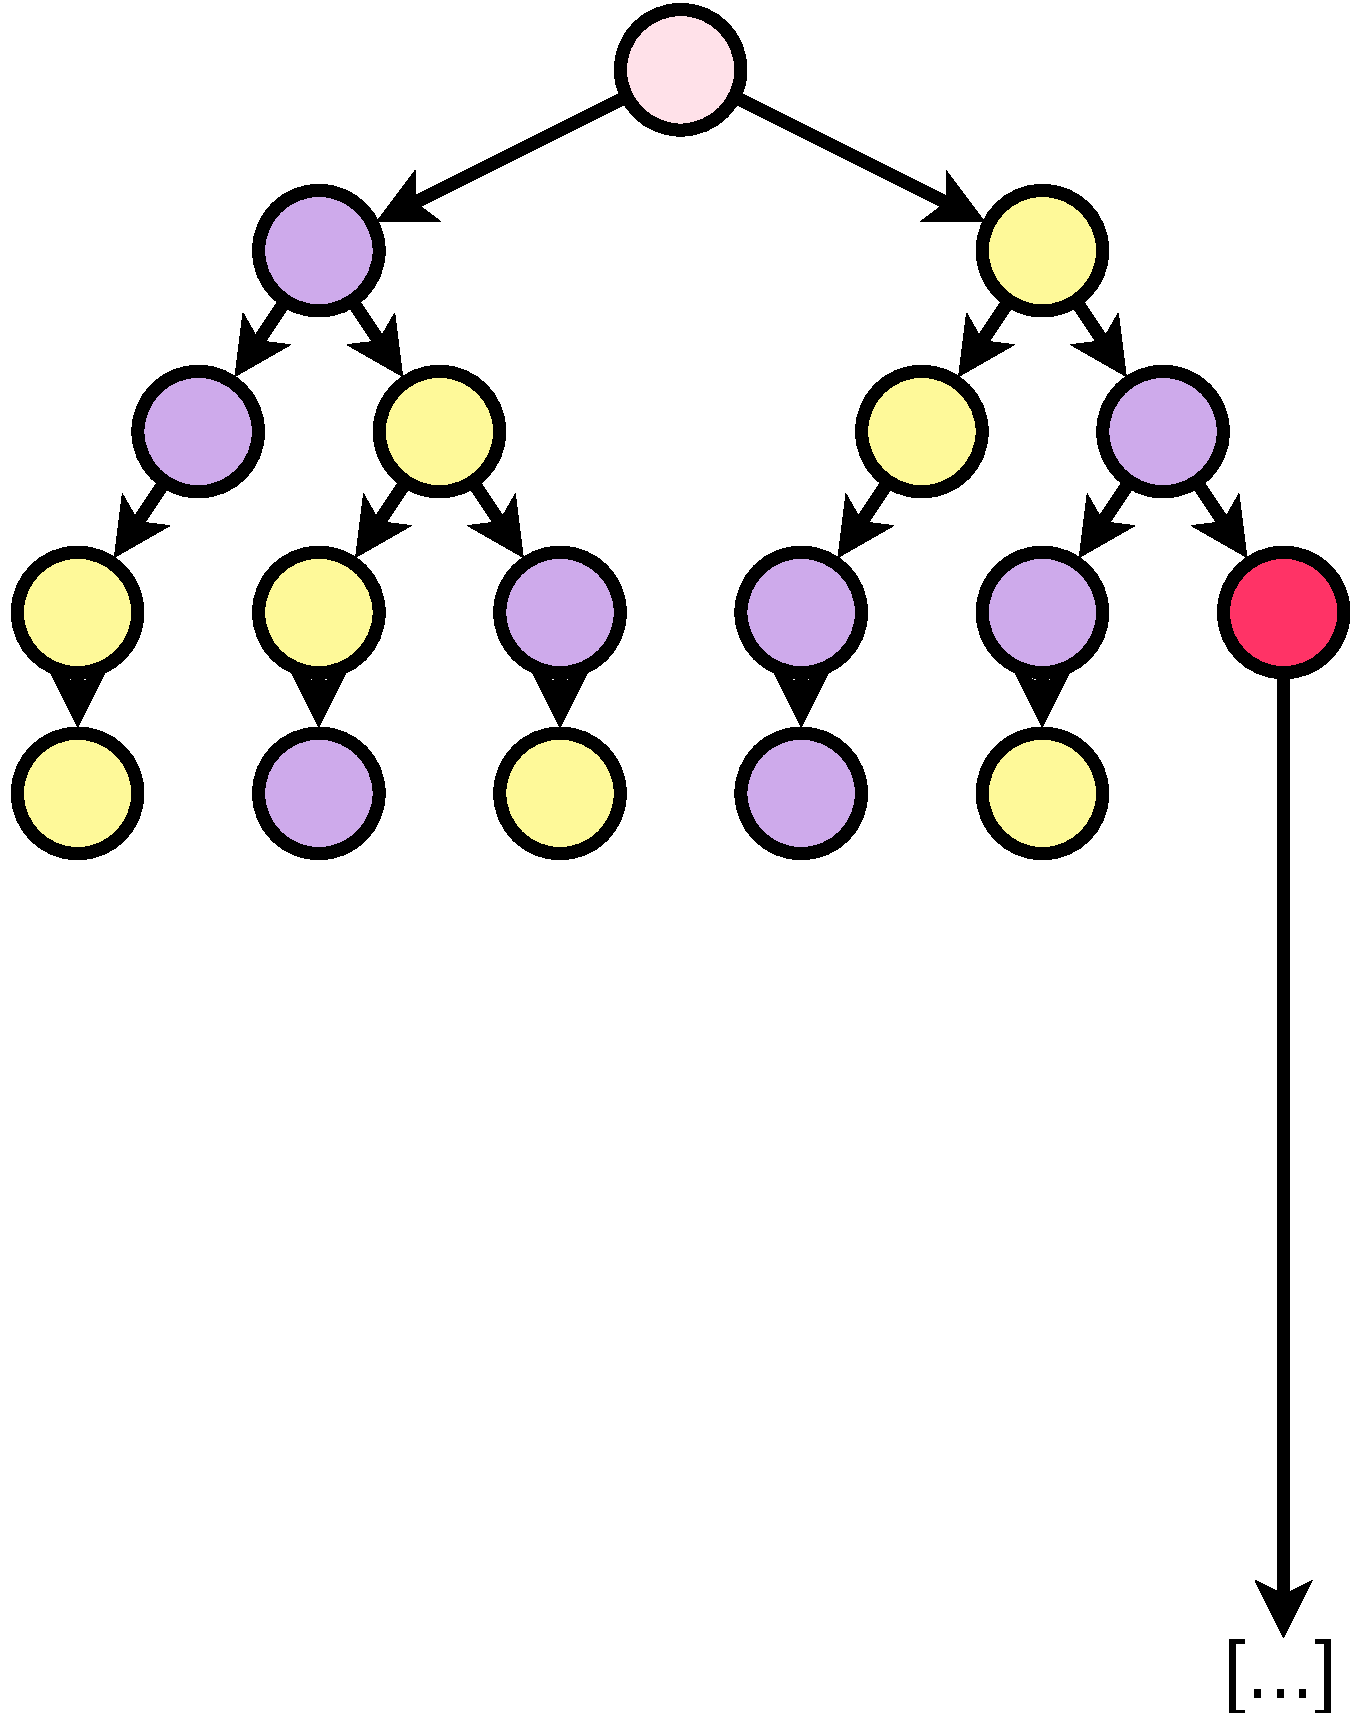
\includegraphics[width=0.28\textwidth]{heuristic-tightloop.pdf}
			\\
			(a) Infinite loop around preemption points.
			&
			(b) Stuck between preemption points.
		\end{tabular}
	\end{center}
	\caption{Detecting infinite loops heuristically by comparison to past interleavings.}
	\label{fig:heuristic-loop}
\end{figure}

Landslide checks for two distinct categories of \revisionminor{potentially-infinite} loops,
visualized in \Cref{fig:heuristic-loop}.
Firstly, it keeps a running average of how many preemption points deep each completed interleaving has been in the past.
Whenever a new preemption point is reached, Landslide checks
if its depth is greater than the heuristic constant factor of 20
({\tt PROGRESS\_DEPTH\_\allowbreak{}FACTOR})
times the previous average.
If the depth exceeds that cutoff, it reports an infinite loop bug.
Whether this represents a livelock or just a mundane sequential logic bug is for the user to decide.
However, as
different interleavings do
often execute different program logic and vary in length accordingly,
Landslide waits to test 10 interleavings ({\tt PROGRESS\_CONFIDENT\_\allowbreak{}BRANCHES})
before applying this heuristic;
in the case of fewer,
it scales the depth factor by a heuristic exponential factor of 1.1
to represent its lower confidence
({\tt PROGRESS\_BRANCH\_UNCERTAINTY\_EXPONENT}).
In the special case of the first branch ever tested,
Landslide will abort after a fixed preemption point depth limit of 4000 ({\tt TOO\_DEEP\_0TH\_BRANCH})
-- a program with such $N$ would probably have an impossibly large state space anyway.

Secondly, a program may get stuck in a loop where no preemption points are encountered each new iteration.
For example, race-induced data corruption may cause a list to end up circularly linked, %oops
leading a search or append operation to fail to terminate.
Landslide also maintains a running average of instructions per transition,
and each instruction, compares if more instructions have elapsed since the last preemption point
than a constant times that average.
Because transitions may themselves vary greatly in number of instructions as each represents completely different program logic,
this heuristic is much more lenient than the preemption-point-counting one,
using a multiplicative factor of 4000 ({\tt PROGRESS\_TRIGGER\_FACTOR}).
If such a loop is encountered within the P2 synchronization primitives,
which should generally be free of $O(n)$ operations,
Landslide uses a more aggressive cutoff of 2000
({\tt PROGRESS\_AGGRESSIVE\_TRIGGER\_FACTOR}).
Also, as transitions between data-race preemption points may have as few as 1 instruction each,
Landslide caps the average from below at a minimum of 1000 ({\tt PROGRESS\_MIN\_TRIGGER\_AVERAGE})
to keep the average relatively stable.
%(100 was found, empirically, to be not enough).

These checks are both implemented in {\tt check\_infinite\_loop()} in {\tt landslide.c}.

\subsubsection{Yield-loop detection}

One very common student implementation pattern in P2s and kernels is to open-code
synchronization between threads using a loop that spins around a condition that the loop itself cannot fulfill,
waiting for another thread to allow it to proceed,
rather than using the established synchronization API.%
\footnote{Even when the student doesn't open-code any such synchronization and always uses {\tt deschedule}
or primitives built thereupon,
{\tt mutex\_test} (\cref{sec:education-pebbles-tests})
often relies on this functionality, as data-race preemption points within {\tt mutex\_lock()}
would otherwise disrupt Landslide's ability to recognize blocking on a contended lock.}
If Landslide failed to recognize that the thread was in principle blocked,
just as if it had called {\tt deschedule} or {\tt cond\_wait()},
this would result in an infinitely deep branch
as it keeps trying to schedule the waiting thread,
blocking all of its attempted context switches to the thread that could make progress.
These loops need not necessarily {\tt yield} each iteration:
they may spin blindly,
assuming progress is being made on another CPU,
which is not possible under Landslide as it serializes execution.

Landslide detects such ad-hoc {\em yield-loop blocking}
by keeping a counter for each thread to track how many {\tt yield}s it has invoked since the last ``interesting'' activity.
% nb. not system calls, not even d/mr, as some student mutexes may use those and you don't want to count them
``Interesting'' here is defined heuristically as any other known P2 API call,
with the exception of {\tt mutex\_lock()} and {\tt mutex\_unlock()}.%
\footnote{Landslide must recognize yield-blocking loops that contain mutex operations
to allow for open-coded reimplementations of {\tt cond\_wait()},
% see comment above "USER_MUTEX_YIELD_ACTIVITY" in user sync.c
which for example the {\tt paraguay} test uses intentionally,
because it is testing the correctness of the student's {\tt cond\_wait()}.}
Whenever this counter reaches the heuristic cutoff of 10 ({\tt TOO\_MANY\_YIELDS}),
Landslide declares the thread blocked,
and treats it just as if it had invoked {\tt deschedule()} for purposes of DPOR
({\tt check\_user\_yield\_activity()} in {\tt user\_sync.c}).
% this also involves propagating yield-blockedness back up the branch, along those 10 pps where it was still counting up to 10
% and also refusing to run any other threads while yield is going on - KEEP_RUNNING_YIELDING_THREADS
%
In cases where {\tt yield} itself is not involved,
Landslide also counts the number of atomic instructions ({\tt xchg}, {\tt xadd}, {\tt cmpxchg}, etc),
and marks the thread blocked if it exceeds 100 such ({\tt TOO\_MANY\_XCHGS\_TIGHT\_LOOP}).%
\footnote{If preemption points exist in between, instead only 20 such ({\tt TOO\_MANY\_XCHGS\_WITH\_PPS}),
to avoid stressing DPOR's $O(n)$ independence computation.}
When such a loop contains neither {\tt yield} nor atomics,
Landslide falls back on the standard infinite loop detector and reports a bug directly, as described above.
Future work could extend this to include more modern ways of establishing memory safety such as
acquire/release barriers
%\cite{sully-thesis}
and hardware transactions.

In order to detect when a thread should be unblocked from its yield loop,
Landslide simply leverages DPOR's existing computation of memory conflicts:
whatever condition the blocked thread was waiting for
will show up in the conflicts between it and whichever thread fulfills it.
Hence, every memory conflict detected during DPOR is also checked against any
currently yield-loop-blocked threads, unblocking them in the case of a match
({\tt check\_unblock\_yield\_loop()} in {\tt user\_sync.c}).
If that memory access is not sufficient to let the blocked thread start making progress again,
it will simply trigger the yield-blocking heuristic again.
In theory, this could result in a livelock between two threads,
each in principle blocked in a yield loop,
but where the conditions of the loop happen to conflict with each other,
causing the threads to keep waking each other up;
however,
% hmm... is this true? like if they use mutexes on each other or smth, or use HTM to check a condition
% where the htm failure path uses a stop the world thing...
I have never observed this in practice, as the conditions \revisionminor{checked by} such blocking loops are usually read-only.
Future work could heuristically address this by deprioritizing such threads,
as measured by the number of times they've yield-blocked,
so that a third thread which could actually make progress may run if it exists.

% mutex learning
% to unblock from open coded accesses in eg unlock_and_vanish
% this is more for blocked_on_addr stuff, not yield blocked stuff
% kind of clunky and uninteresting to talk abt tbh

\subsubsection{False-positive deadlock avoidance}

In cases where the yield-loop heuristic described above produces false positives,
i.e., blocking a thread which could make progress on its own after all,
Landslide must avoid reporting a deadlock bug if no other thread ends up waking it up through memory conflicts.
After all other threads quiesce,
which ordinarily would trigger deadlock detection,
Landslide checks the system for any yield-looping threads that were blocked heuristically.%
\footnote{This includes threads blocked on specific mutexes using the {\tt blocked\_on\_addr} field,
which is set when {\tt yield} is invoked within {\tt mutex\_lock()} without waiting for 10 loops.}
If any exist, it forces them awake and allows them to proceed;
if they are truly blocked in principle,
they will merely trip the yield-loop limit and go back to sleep again,
\revisionminor{whereupon Landslide will issue a deadlock bug report after all.}

Two other forms of heuristic blocking exist in Landslide which are also subject to this retry procedure.
Firstly, when an interleaving has already exhausted the number of preemptions allowed under ICB's current bound,
other threads which are runnable but which require preemptions to switch to are considered ``ICB-blocked''.
When yield-looping mixes with ICB-blocking, the yielding thread will require a preemption
for the other thread to fulfill its blocking condition.
In such a case, simply spending all 128 deadlock-avoidance retries on the yield-looping thread will not solve anything,
so the ICB-blocked thread must be forced awake with higher priority,
disregarding the preemption bound,
to allow the system to progress.
Secondly, in programs which use HTM,
threads blocked by retry sets (\cref{sec:tm-retrysets})
must be forced awake with priority before yield-blocked threads,
along similar reasoning.

Landslide will retry this process up to a heuristic limit of 128 times ({\tt DEADLOCK\_FP\_MAX\_\allowbreak{}ATTEMPTS}
before issuing a deadlock bug report.
The overhead of this check is quadratic time in the number of retries permitted
(as DPOR is quadratic in the overall branch depth),
although this is negligible compared to the exponential size of state spaces overall.
If the heuristic limit is too small, very ``loopy'' programs
(which invoke xchg or yield therein)
could falsely exhaust this limit while not being truly deadlocked,
so a good limit should be well higher than the total number of concurrency events expected for any Landslide-friendly test.
The cost of a high limit manifests in the length of preemption traces when deadlock is declared,
which will display a proportional number of meaningless preemption points,
although future work could easily truncate them retrospectively.
This check is implemented in {\tt try\_avoid\_fp\_deadlock()} in {\tt arbiter.c}.
